% =====================================================================
% SS-RESfM — CVPR 2027 submission draft (ported from ICLR_ssresfm.tex Sep 6 2026)
% CVPR 2027: 8 pages INCLUDING figures/tables; references unlimited; double-blind.
% TODO before submission: replace cvpr.sty with the official CVPR 2027 Author Kit
% version and set the real Paper ID. [review] adds ruler + ID.
% =====================================================================
\documentclass[10pt,twocolumn,letterpaper]{article}
\usepackage[review]{cvpr}
\usepackage{times}
\usepackage{graphicx,amsmath,amssymb,booktabs,multirow,xcolor}
\usepackage[pagebackref,breaklinks,colorlinks]{hyperref}
\def\confName{CVPR}
\def\confYear{2027}
\newcommand{\mad}{\textsc{madweight}}
\renewcommand{\deg}{^{\circ}}
\def\paperID{*****}
\title{When Outlier Supervision Fails: Supplementary Material}
\author{Anonymous CVPR submission\\ Paper ID *****}

\begin{document}
\maketitle
\appendix
\subsubsection*{Reproducibility Statement}
All results are reproducible from the released materials: code (a documented fork of
RESfM's public repository), every training and evaluation configuration file, the
rebuilt track suites for the five OOD datasets and the per-domain train/val/test splits of the main paper's in-distribution study, and the scripts that regenerate every table and figure from the
saved evaluation outputs (including a verification script that recomputes each printed
cell). Training protocol, learning rates, schedules, and checkpoint-selection rules are
specified in the main paper's protocol section; seeds are enumerated per experiment ($20$--$24$),
and every headline comparison reports five-training-seed bands. Sources of
irreducible run-to-run variance (robust-BA solver nondeterminism, TTT) are
characterized in the supplementary so that deviations within those bounds can be
recognized as environmental. Dataset provenance and licences: all datasets are public
academic benchmarks; our track builder and download manifests are included.

\subsubsection*{Ethics Statement}
This work studies robustness of 3D reconstruction on standard public benchmarks of
landmark photographs (MegaDepth, 1DSfM, Strecha, BlendedMVS, Olsson's dataset) and
introduces no new data collection, no personal data processing beyond what those
established benchmarks already contain, and no human subjects. Improved robust SfM has
broadly beneficial applications (mapping, cultural heritage, robotics); we are not
aware of ethical concerns specific to this method beyond those generic to 3D
reconstruction of public imagery.


\section{Full 1DSfM-hard mechanism table}
\begin{table}[h]\centering\small
\caption{\textbf{1DSfM-hard} ($\sim\!60\%$ outliers, seed 20): translation/rotation
and registered fraction.}
\label{tab:hard}
\begin{tabular}{lcc}
\toprule
Method & Trans/Rot (post-BA) & Registered\\
\midrule
remove & $\mathbf{10.6}$/$\mathbf{12.4}$ & all\\
\mad{} & 12.2/14.4 & all\\
remove+TTT & 15.2/16.8 & all\\
RESfM-scratch              & 16.2/22.7 & all\\
huberweight & 16.9/24.5 & all\\
COLMAP                     & 20.9/--   & 64\%\\
weight & 21.9/25.6 & all\\
stdweight & 23.2/27.3 & all\\
hybrid & 26.3/28.7 & all\\
weight+TTT & 26.4/32.0 & all\\
\bottomrule
\end{tabular}
\end{table}

\section{Rotation and registration panels of the main comparison}\label{app:rotnr}
Rotation errors and registered-camera fractions for every arm of the main comparison
(Table~2 of the main paper); conventions as there.
\begin{table}[h]\centering\footnotesize\setlength{\tabcolsep}{3pt}
\resizebox{\linewidth}{!}{\begin{tabular}{lcccccc}
\toprule
Arm & MegaDepth & 1DSfM & 1DSfM-hard & Strecha & BMVS & Olsson\\
\midrule
\multicolumn{7}{l}{\emph{Rotation error ($\deg$, five-seed means; classical row single run)}}\\[1pt]
\mad{}       & 3.70 & 7.74 & 27.7 & 12.80 & 9.01 & 14.4\\
weight       & 3.28 & 8.24 & 28.0 & 7.61 & 9.17 & 13.2\\
weight+TTT   & 2.88 & 10.09 & 30.6 & 7.95 & 8.30 & 11.6\\
remove       & 4.04 & $\mathbf{6.94}$ & $\mathbf{12.3}$ & 14.39 & 16.04 & 13.9\\
remove+TTT   & 4.22 & 6.90 & 16.4 & 13.23 & 13.19 & 14.5\\
GLOMAP (classical)          & 5.30 & 8.78 & 26.4 & 0.25 & $\mathbf{2.15}$ & $\mathbf{1.29}$\\
RESfM-scratch (supervised)  & $\mathbf{1.89}$ & 9.62 & 27.3 & $\mathbf{1.56}$ & 31.66 & 12.6\\
\midrule
\multicolumn{7}{l}{\emph{Registered cameras $N_r/N_c$ (five-seed means; classical row single run)}}\\[1pt]
\mad{}       & 81\% & 70\% & 43\% & 91\% & 92\% & 86\%\\
weight       & 79\% & 79\% & 40\% & 98\% & 94\% & 90\%\\
weight+TTT   & 77\% & 81\% & 41\% & 99\% & 94\% & 90\%\\
remove       & 72\% & 58\% & 29\% & 97\% & 88\% & 78\%\\
remove+TTT   & 71\% & 58\% & 32\% & 96\% & 90\% & 78\%\\
RESfM-scratch (supervised)  & 85\% & 77\% & 34\% & 99\% & 92\% & 89\%\\
GLOMAP (classical)          & $\mathbf{96}$\% & $\mathbf{96}$\% & $\mathbf{80}$\% & $\mathbf{100}$\% & 86\% & $\mathbf{100}$\%\\
\bottomrule
\end{tabular}}
\end{table}

\begin{figure}[h]\centering
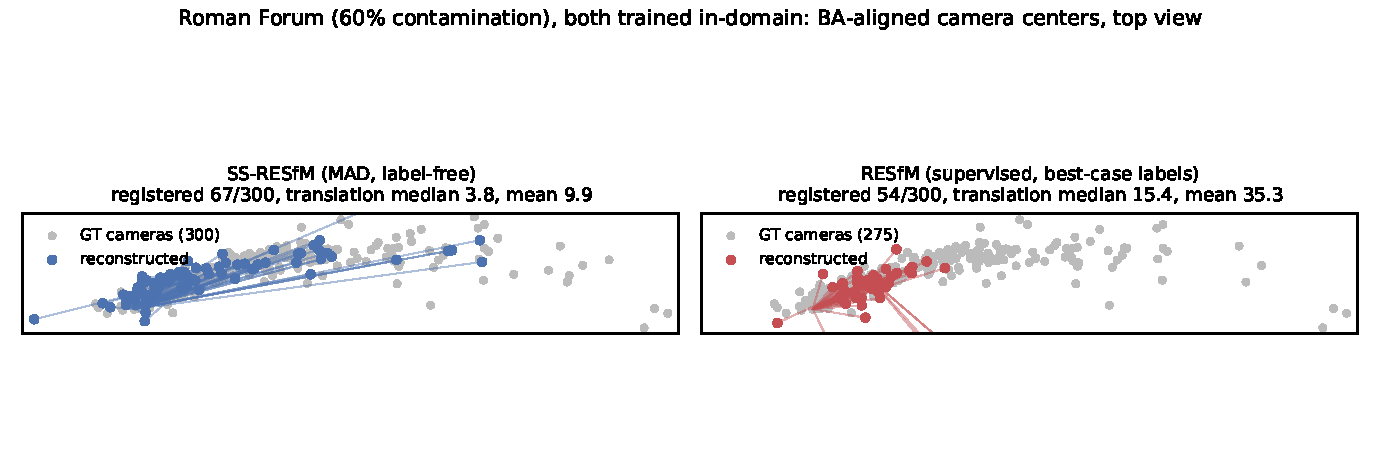
\includegraphics[width=\linewidth]{fig_qual_romanforum.pdf}
\caption{\textbf{Qualitative view of the $60\%$ label ceiling} (Roman Forum, seed
$20$, both recipes trained in-domain, supervised with GT-derived labels): BA-aligned
camera centers in top view; whiskers join each reconstructed camera to its ground-truth
position. The label-free \mad{} arm (left) registers more cameras ($67$ vs.\ $54$ of
$300$) that track the ground-truth layout at a usable median error ($3.8$ vs.\
$15.4$), while the supervised reconstruction (right) collapses toward a compressed
cluster with large systematic displacements --- supervision fails here \emph{with the
best labels it could ever have}.}
\label{fig:qualrf}
\end{figure}

\section{Training-pool diversity and the label ceiling}\label{app:diversity}
A preliminary experiment (single seed, under a coarser five-milestone decay schedule;
cf.\ the main paper's protocol section) retrains both methods on progressively diversified pools: MegaDepth-27
$\to$ $+$ETH3D ($39$ scenes, added data ${\sim}8\%$ contaminated) $\to$ $+$VGG/T\&T ($52$
scenes, adding a ${\sim}16\%$-contaminated mid-band). The supervised baseline's clean-OOD
accuracy degrades \emph{monotonically} with diversity (Strecha
$0.006\!\to\!0.77\!\to\!2.83$); in distribution the same diversification is nearly
free (MegaDepth $0.33\!\to\!0.32\!\to\!0.44$, the first step within noise), so the
collapse is specific to clean OOD generalization, not a general capacity cost. Meanwhile the clean addition yielded no high-contamination
gain and only the contaminated mid-band coincided with one (1DSfM $11.0/11.5/8.8$;
differences within single-seed noise on this benchmark, so consistent with, though not
established by, these runs). If it holds, the implication is pointed: the data that
helps is precisely the data whose COLMAP labels degrade (cf.\ the label ceiling), making
supervised diversity scaling self-limiting.

A four-cell control (single seed each, canonical schedule) sharpens the architecture
question: on the Olsson clean benchmark, the supervised collapse persists for a
\emph{deep} network on the MegaDepth-only pool ($8.58$) and for a \emph{shallow} network
on the diversified $52$-scene pool ($9.30$), yet vanishes for deep networks on the
diversified pool ($2.26$ plain; $2.83$ with LayerNorm/residual --- so normalization is
not the ingredient). Neither capacity nor data diversity alone rescues the supervised
recipe; only their combination does. The label-free arms reach the same level
($2.9$--$3.6$) from the \emph{shallow, single-pool} configuration --- the cheapest cell
of the grid --- which reframes the comparison: self-supervision buys at $1{\times}3$
capacity on $27$ scenes what supervision needs both depth and a curated multi-dataset
pool to approach.

A two-stage control sharpens what kind of failure the collapse is. Retraining the
supervised recipe from scratch on tracks pre-cleaned by its own best outlier head (with
label-free reprojection-based checkpoint selection) does nothing at the full $20$k+$20$k
budget --- all five seeds collapse ($8.3$--$12.0$) --- but a \emph{compute-matched}
$10$k+$10$k version escapes in three of five seeds ($1.69$/$2.01$/$2.29$, matching the
best cells of the grid) while the other two collapse ($7.8$/$12.1$), with the same
bimodality on Strecha ($0.01$--$0.2$ vs.\ $1.9$/$2.4$). The good basin is therefore
\emph{reachable} from the shallow single-pool configuration --- the collapse is basin
selection, not a capacity or data impossibility --- but no supervised-lineage recipe we
tested reaches it reliably: across seeds, clean-OOD reliability is delivered only by the
label-free arms and by depth$\times$diversity. Nor do the two remedies compose: applying
the same two-stage cleaning \emph{on top of} the depth$\times$diversity configuration
destroys its fix (Olsson $9.94$ vs.\ $2.83$ one-stage) --- pre-cleaning strips the very
training signal the diverse pool provides --- while incidentally producing the best
BlendedMVS result in the study ($0.10$). Data surgery and data diversity are
substitute-seeking interventions that interfere, not stack. The
label-free arms diverge by mechanism, and the canonical-schedule three-seed replication
(authors' configuration, $52$ scenes) now separates the robust from the fragile:
\mad{}'s clean-OOD diversity-robustness is seed-stable (BlendedMVS $0.12\pm0.01$ vs.\
the baseline's $0.35\pm0.04$), whereas its high-contamination gain is real only in the
best case: 1DSfM $5.4/11.2/12.8$ across seeds ($9.8\pm3.9$), overlapping the
single-pool band ($11.5\pm2.3$). Diversification can yield large gains at $43\%$ but
does not do so reliably, and yields none at $60\%$ ($20.1\pm1.2$); soft weighting
collapses on clean OOD like the baseline at the retired schedule ($2.9$--$4.0$) and
holds only BlendedMVS under the canonical one.

\section*{Schedule robustness (from main protocol)}
\noindent\textbf{Schedule robustness.} All reported results use RESfM's released
eleven-milestone schedule. An earlier accidental five-milestone variant of ours was
retired; a three-seed replication of \emph{both} schedules shows the schedule effect lies
within seed noise (MegaDepth $0.46\pm0.08$ vs.\ $0.40\pm0.09$; 1DSfM $9.6\pm3.2$ vs.\
$12.2\pm2.4$, per-seed rankings inverting on both), with mechanism orderings stable
throughout.


\section{Qualitative results}\label{app:qual}
Fig.~\ref{fig:qual} overlays BA-aligned camera centers on ground truth for 1DSfM
NYC\_Library. Label-free \mad{} ($2.94$) leaves far fewer gross-drift cameras than the
supervised from-scratch baseline ($6.28$), which shows more and larger gross drifts.

\begin{figure}[t]
\centering
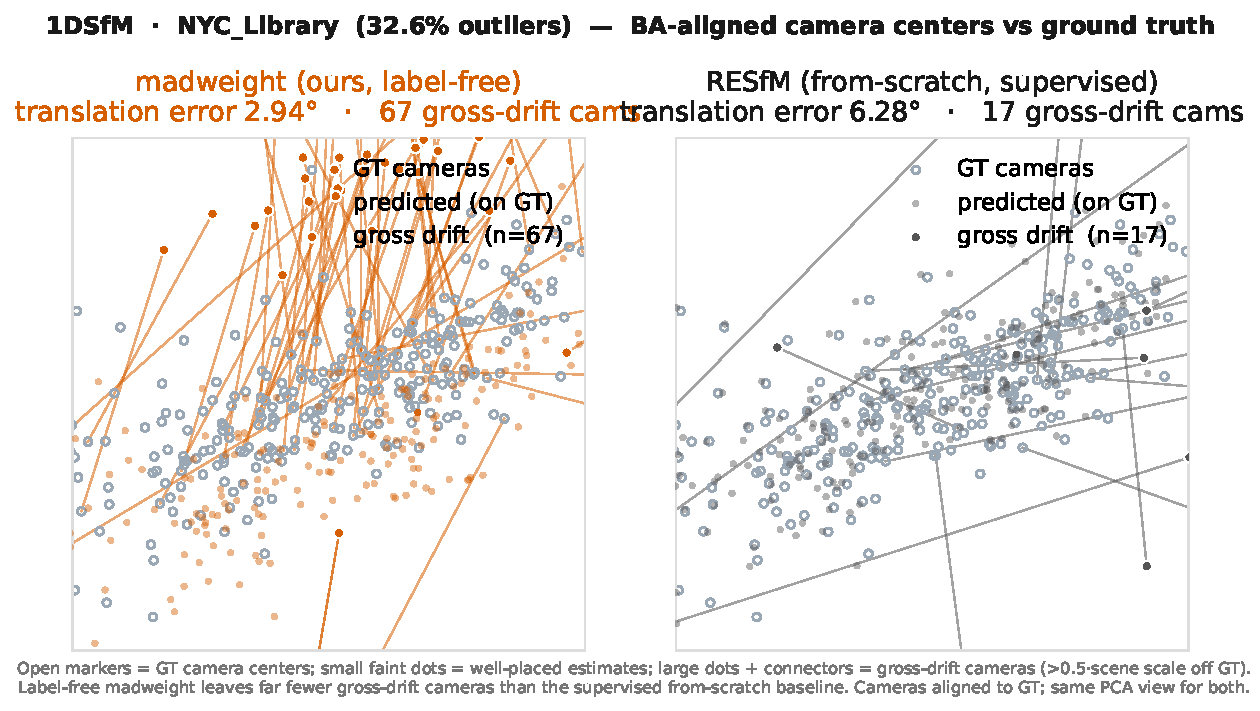
\includegraphics[width=\linewidth]{PATHA_fig3_qualitative.pdf}
\caption{\textbf{Qualitative 1DSfM (NYC\_Library, 32.6\% outliers).} BA-aligned camera
centers vs.\ GT (open markers); large dots\,+\,connectors mark gross-drift cameras. \mad{}
(left, $2.94$) has fewer and shorter drifts than RESfM-from-scratch (right, $6.28$).}
\label{fig:qual}
\end{figure}


\section{Learning-rate robustness of the baseline}\label{app:lrgrid}\label{sec:lrgrid}
Our protocol gives each method its best learning rate at the canonical $20$k budget
($10^{-3}$ for the supervised arms, RESfM's released value; $10^{-4}$ for the
self-supervised arms). To test how much the conclusions depend on this choice we trained
the supervised baseline at $10^{-4}$ as well. In distribution the released value is
clearly right ($0.344$ vs.\ $0.533$), and at $10^{-4}$ the supervised model is
truncation-limited (best checkpoint at the final epoch). Out of distribution, however,
the picture splits: the baseline's Olsson collapse persists at \emph{both} rates
($8.47$ vs.\ $8.54$), i.e.\ the clean-benchmark supervised failure is lr-robust,
whereas its BlendedMVS, 1DSfM, and 1DSfM-hard deficits shrink substantially at the lower
rate ($0.379\!\to\!0.139$, $11.0\!\to\!5.9$, $16.2\!\to\!12.8$): the
under-trained low-rate model overfits MegaDepth less and generalizes better. Two follow-ups
complete the grid. A $30$k-budget replicate at $10^{-4}$ plateaus (best validation at
epoch $16$k, never improving through $30$k), and its evaluation sharpens the picture:
that checkpoint reaches \emph{near-parity in distribution} ($0.365$ vs.\ the $10^{-3}$
baseline's $0.344$) while keeping the OOD gains (1DSfM $6.1$, 1DSfM-hard $13.9$,
BlendedMVS $0.18$), making it the strongest supervised variant out of distribution
(single seed). The Olsson ($8.27$) and Strecha ($1.64$) failures persist, and label-free
plain removal still leads at extreme contamination ($12.4\pm2.1$ vs.\ $13.9$); the OOD
advantage of the low rate is a regularization effect, not an under-training artifact. And the self-supervised
arms show \emph{no} symmetric effect: trained at $10^{-3}$ they are worse on every
dataset (madweight MegaDepth $0.75$ vs.\ $0.42$, 1DSfM $15.7$ vs.\ $12.4$, Olsson
$10.1$ vs.\ $2.6$). Each method's declared rate is therefore its empirical best-of-two,
and the off-rate OOD gain is specific to supervision, consistent with a
COLMAP-label-fitted classifier overfitting in distribution. We scope our claims
accordingly: the Olsson and Strecha findings and the mechanism flip itself are
lr-robust, while the magnitude of the supervised OOD deficit at BlendedMVS and high
contamination depends on the baseline's learning rate.


\section{Full mechanism matrix}\label{app:matrix}
Table~\ref{tab:matrix} completes the mechanism study (all arms, RESfM-aligned schedule,
seed 20). Notably, at $43\%$ the \emph{plain-removal} family leads every arm including the
supervised baseline, and the full three-seed band confirms it: remove+TTT
$8.7\pm1.1$ mean (every seed below the baseline's $11.0$), plain remove median
$1.59\pm0.18$ (vs.\ $2.9$; means $9.1\pm2.8$, dominated by the two failure scenes). On
clean data the soft arms dominate the removal family, reproducing the complementarity.
On outlier-free Olsson the grid flattens (all label-free arms $2.6$--$4.1$ vs.\
supervised $8.5$): the clean-benchmark failure is specific to the supervised head, not
the mechanism.

\begin{table}[t]\centering\scriptsize
\setlength{\tabcolsep}{2.5pt}%
\caption{\textbf{Full shallow mechanism matrix} (RESfM-aligned schedule, seed 20;
$^{\ddagger}$mean$\pm$std over seeds 20--22). Mean\,/\,median translation
(post-BA); Olsson column: means. Best per column in \textbf{bold}.}
\label{tab:matrix}
\resizebox{\linewidth}{!}{%
\begin{tabular}{lccccc}
\toprule
Arm & MD & 1DSfM & Strecha & BMVS & Olsson\\
\midrule
remove       & 0.60/0.19 & 9.1$\pm$2.8/$\mathbf{1.6\pm 0.2}$$^{\ddagger}$ & 3.02/1.68 & 0.27/0.19 & 2.81\\
remove+TTT   & 0.49/0.13 & $\mathbf{8.7\pm 1.1}$/2.2$\pm$1.1$^{\ddagger}$ & 2.97/1.56 & 0.19/0.07 & 4.07\\
hybrid       & 0.37/0.20 & 16.0$\pm$1.4/6.7$\pm$4.4$^{\ddagger}$ & 2.70/1.39 & 0.10/0.03 & 2.82\\
hybrid+TTT   & 0.39/0.14 & 15.4$\pm$1.1/10.7$\pm$3.5$^{\ddagger}$ & 3.52/2.65 & 0.13/$\mathbf{0.00}$ & 3.19\\
\mad{}       & 0.42/0.15 & 11.5$\pm$2.3/6.0$\pm$1.4$^{\ddagger}$ & 2.50/0.97 & 0.15/0.004 & $\mathbf{2.57}$\\
weight       & 0.42/0.18 & 15.8$\pm$3.1/10.9$\pm$2.1$^{\ddagger}$ & 2.00/0.03 & $\mathbf{0.10}$/0.04 & 2.65\\
weight+TTT   & 0.39/0.14 & 17.0$\pm$1.3/10.9$\pm$4.1$^{\ddagger}$ & 1.98/$\mathbf{0.005}$ & 0.14/0.01 & 7.74\\
\midrule
RESfM (sup.) & $\mathbf{0.34/0.07}$ & 11.03/2.93 & $\mathbf{0.006/0.005}$ & 0.38/0.35 & 8.47\\
\bottomrule
\end{tabular}}%
\end{table}


\section{Which robust statistic? MAD vs.\ STD vs.\ Huber}\label{app:stat}
\mad{} removes by a robust statistic of the reprojection error; we ablate the statistic
holding the head reweighting fixed: MAD (median${}+\alpha\cdot1.4826\,$MAD, $50\%$
breakdown), a Huber M-estimate of scale (IRLS), and non-robust STD
(mean${}+\alpha\sigma$), all at $\alpha{=}2$. Table~\ref{tab:madstat} reports the
ablation over seeds $20$--$22$: only MAD's 1DSfM median is stable; Huber's collapses on
one seed, and non-robust STD is consistently poor, its mean/$\sigma$ threshold inflated
by the very outliers it should catch. On clean data all three are comparable: little is
removed either way, the right behavior without outliers. The $50\%$-breakdown statistic
is the only reliably robust choice, and we use MAD in \mad{}.

\begin{table}[t]\centering\scriptsize
\setlength{\tabcolsep}{2.5pt}%
\caption{\textbf{Removal-statistic ablation} (head reweighting fixed). Only MAD's
median is seed-stable.}
\label{tab:madstat}
\begin{tabular}{lccc}
\toprule
Statistic & 1DSfM mean & 1DSfM med.\ s20/21/22 & BMVS\\
\midrule
MAD (\mad{}) & 11.5$\pm$2.3 & $\mathbf{4.4\,/\,7.0\,/\,6.6}$ & 0.15\\
Huber & $\mathbf{11.5\pm 1.6}$ & 3.8 / 12.4 / 5.3 & $\mathbf{0.11}$\\
STD & 15.2$\pm$1.2 & 13.3 / 9.0 / 12.9 & 0.15\\
\bottomrule
\end{tabular}
\end{table}



\section{Sensitivity of the self-supervision hyperparameters}\label{app:hyper}
SS-RESfM introduces two hyperparameters: the pseudo-label percentiles (default
$20/80$) and the removal threshold ($\tau{=}0.6$, RESfM's released value). Both were
fixed a priori, not tuned per dataset; this appendix reports their sensitivity.

\noindent\textbf{Removal threshold.} Sweeping $\tau\in\{0.4,\dots,0.8\}$ on the
default-percentile checkpoint (seed 20): MegaDepth varies only $0.38$--$0.58$
(flat within $0.38$--$0.43$ for $\tau\ge0.5$), Strecha $3.06$--$3.22$, BlendedMVS
$0.20$--$0.27$, and 1DSfM $7.97$--$10.35$ with no consistent optimum; the default
$\tau{=}0.6$ is never far from the per-dataset best. The threshold is a non-issue.

\begin{table}[t]\centering\footnotesize
\caption{\textbf{Hyperparameter sensitivity} (seed 20, single runs; earlier
five-milestone schedule for the percentile variants). Left: pseudo-label percentiles.
Right: removal threshold $\tau$ on the default checkpoint. Mean translation.}
\label{tab:hyper}
\setlength{\tabcolsep}{4pt}%
\begin{tabular}{lcc@{\hskip 18pt}lcc}
\toprule
Percentiles & MD (weight) & 1DSfM (\mad{}) & $\tau$ & MD & 1DSfM\\
\midrule
10/90 & 0.49 & 13.0 & 0.4 & 0.58 & \phantom{0}8.0\\
15/85 & 0.51 & 15.6 & 0.5 & 0.40 & 10.4\\
20/80$^{*}$ & 0.42 & 12.4 & 0.6$^{*}$ & 0.39 & \phantom{0}9.1\\
25/75 & 0.60 & 14.9 & 0.7 & 0.38 & \phantom{0}9.7\\
30/70 & 0.44 & \phantom{0}8.8 & 0.8 & 0.43 & 10.0\\
\bottomrule
\end{tabular}
\end{table}

\noindent\textbf{Pseudo-label percentiles.} Across a $4\times$ range of percentile
choices (Table~\ref{tab:hyper}), in-distribution accuracy is flat
(MegaDepth $0.42$--$0.60$), and 1DSfM varies by $\pm3$--$6$ --- an amount comparable to
the training-seed bands of Table~2 of the main paper ($\pm1.7$--$3.0$), with no setting
consistently best across mechanisms (these are single-seed cells, so part of the spread
\emph{is} seed noise). The default $20/80$ sits mid-range everywhere and was chosen
before any evaluation. We conclude the method is not sensitively tuned: neither knob,
varied broadly, moves results beyond the seed-level noise this paper quantifies
everywhere else.

\section{Per-scene complementarity and the limits of contamination-based selection}\label{app:selector}
Fig.~\ref{fig:perscene} tests the flip \emph{per scene}: each scene's outlier rate vs.\
the signed advantage of the best removal mechanism over soft weighting. On OOD data,
weight wins the low-contamination scenes and removal the high-contamination ones; the
crossover is bracketed to the sparsely-sampled ${\sim}3$--$29\%$ band.

\begin{figure}[t]
\centering
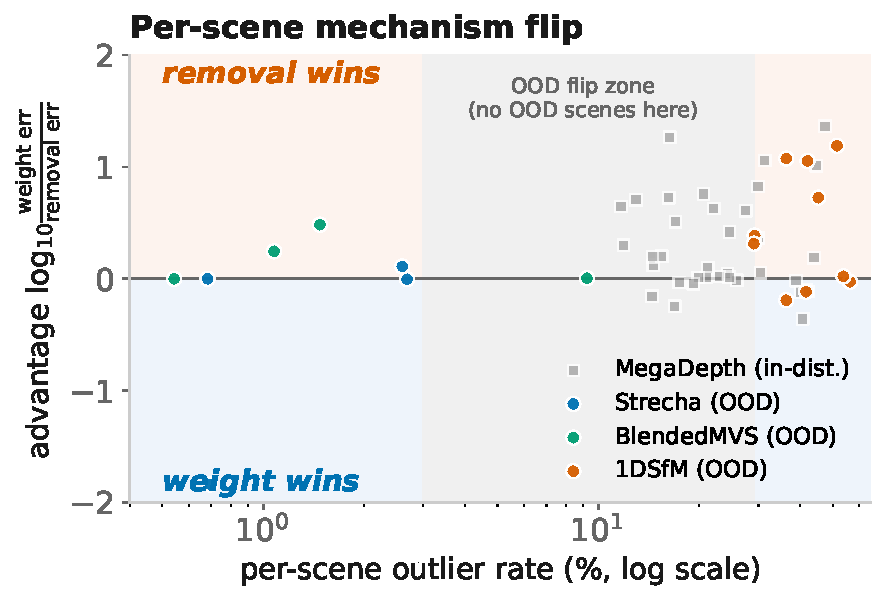
\includegraphics[width=\linewidth]{PATHA_fig4_perscene.pdf}
\caption{\textbf{Per-scene complementarity} (RESfM-aligned schedule). Each point is one
scene: outlier rate (x, log) vs.\ signed advantage of removal over soft weighting. Weight
wins at low contamination, removal at high contamination.}
\label{fig:perscene}
\end{figure}

\noindent\textbf{Does per-scene contamination help selection?} No: within each dataset
contamination is too homogeneous to trigger different choices, so a contamination-keyed
selector (\mad{} if scene rate ${\ge}10\%$, else weight) collapses to per-dataset
selection (Table~\ref{tab:selector}). An \emph{oracle} choosing the best of five
mechanisms per scene from ground-truth error would change the picture: MegaDepth
$0.42\!\to\!0.116$, surpassing every fixed arm, the supervised baseline at $0.344$,
and even RESfM-released at $0.209$, and 1DSfM $12.4\!\to\!5.8$ vs.\ the
baseline's $11.0$. The performance is thus already \emph{latent} in the label-free mechanism family;
selection, not mechanism design, is the bottleneck. A first unsupervised step exists:
running all five mechanisms and keeping the reconstruction with the lowest post-BA
reprojection error reaches $0.276$ on MegaDepth, past every fixed arm and the supervised
baseline ($0.344$), and matches the oracle on BlendedMVS (Table~\ref{tab:selector},
self-sel.). We report this as a secondary observation rather than a claim: it spends
$5\times$ test-time compute, and it inherits reprojection's retention bias exactly where
pruning over-fires (1DSfM $12.8$ vs.\ plain remove's $8.9$). Cheaper selection signals
fail informatively. The classification head cannot estimate contamination at all:
trained on per-scene \emph{percentile} pseudo-labels, it is a rank calibrator, not a
rate estimator, flagging a near-constant $39$--$42\%$ of observations on datasets
whose true contamination spans $0.5$--$60\%$ (this also explains the collapse of
contamination-keyed selection, and retroactively justifies \mad{}'s design choice of
thresholding reprojection statistics rather than head scores). And \emph{pre}-fine-tune
reprojection magnitudes measure domain shift, not contamination (in-distribution
MegaDepth shows the largest raw error); only the \emph{post}-fine-tune residual tracks
the contamination axis monotonically. Realizing the remaining headroom at unit compute
is future work.

\begin{table}[t]\centering\footnotesize
\setlength{\tabcolsep}{3pt}%
\caption{\textbf{Per-scene selection} (mean translation; RESfM-aligned schedule).
Contamination-keyed selection collapses to per-dataset choice. The oracle uses
ground-truth error over five mechanisms: an upper bound, not a deployable method.
Self-sel.: run all five, keep the lowest post-BA reprojection error (unsupervised,
$5\times$ test-time compute); a secondary observation, not a headline method.}
\label{tab:selector}
\begin{tabular}{lccccc}
\toprule
Dataset & weight & madwt & contam & self-sel.\ ($5\times$) & oracle (GT)\\
\midrule
MegaDepth  & 0.423 & $\mathbf{0.422}$ & 0.422 & 0.276 & $\mathit{0.116}$\\
1DSfM      & 12.79 & $\mathbf{12.39}$ & 12.39 & 12.83 & $\mathit{5.78}$\\
Strecha    & $\mathbf{2.00}$ & 2.50 & 2.00 & 2.70 & $\mathit{1.98}$\\
BlendedMVS & $\mathbf{0.100}$ & 0.146 & 0.100 & 0.083 & $\mathit{0.083}$\\
\bottomrule
\end{tabular}
\end{table}


\clearpage
\section{Environment sensitivity and reproducibility of post-BA benchmarks}\label{app:repro}
This appendix reproduces the full study behind the protocol's environment-noise and
stack-replication statements (main paper, protocol section).

\subsection{The reproduction question}\label{sec:repro}
Evaluating the RESfM authors' \emph{released checkpoint} in our harness on the 36 MegaDepth
test scenes yields a post-BA mean translation error of $0.209$ vs.\ the published $0.169$
(rotation $1.89\deg$ vs.\ $1.29\deg$). Since our controlled comparisons hinge on baseline
fidelity, we traced this discrepancy to its source. The finding is of independent
interest: \textbf{dataset-level post-BA means on MegaDepth-scale benchmarks carry a
practical environment-noise floor of $\mathcal{O}(0.05)$ for non-TTT evaluations},
produced by chaotic basin selection in robust bundle adjustment --- and the floor is
larger elsewhere: per-scene values flip by up to $\pm0.37$ (released checkpoint:
$0.043\!\to\!0.892$ on scene 0046), TTT-based cells carry $\sim\!0.14$ mean-level
run-to-run variance (\S\ref{sec:ttt}), and on high-error benchmarks the floor scales
with the error (released checkpoint on 1DSfM: $\pm0.27$ across runs). Third-party
corroboration: the VGPA appendix~\cite{vgpa} reports that re-running RESfM under their
own protocol shifts its numbers because ``the final bundle-adjustment stage is not
fully deterministic'' --- the same environment-noise layer, observed independently by
the original authors' group. This corroborates the noise floor only: the reproduction
gap itself ($0.169$ vs.\ $0.34$--$0.39$, roughly $4\times$ the floor) traces to
\emph{training} (checkpoint provenance and training-seed variance), not to bundle
adjustment.

\begin{table}[h]\centering\footnotesize
\caption{Released RESfM checkpoint, MegaDepth 36-scene post-BA means, under three
conditions, vs.\ the published number. $N_r$ is the mean number of registered cameras
per scene; the published row averages the
paper's per-scene Table~1 values.}
\label{tab:supp_reprocond}
\resizebox{\linewidth}{!}{%
\begin{tabular}{lccc}
\toprule
Condition & Trans & Rot ($\deg$) & $N_r$\\
\midrule
Published (paper Table 1) & 0.169 & 1.29 & 298\\
Our env (pip/OpenBLAS), 5-seed mean & 0.203 & 1.82 & 304\\
Our env, seed 20 & 0.209 & 1.89 & 304\\
Authors' exact stack (conda/MKL) & 0.217 & 1.92 & 304\\
\bottomrule
\end{tabular}}
\end{table}

\subsection{Eliminating the controllable factors}\label{sec:factors}
\noindent\textbf{Data.} Our MegaDepth npz files are byte-identical to the authors' released
archive, including the Group-2 300-camera subsamples.

\noindent\textbf{Randomness.} Five evaluation seeds vary the pre-BA network output by
$\pm 0.004$ and the post-BA mean by $\pm 0.01$; negligible.

\noindent\textbf{Network forward pass.} The pre-BA output (translation/rotation
$\sim\!1.73/11.9\deg$) is essentially seed- and environment-stable; the divergence
therefore enters at the robust-BA stage. (Notably, the paper does not report pre-BA
numbers; all its tables are post-robust-BA.)

\noindent\textbf{Software stack.} We rebuilt the authors' \emph{exact pinned environment}
from their released \texttt{environment.yaml}: Python 3.8.20, MKL-backed numpy 1.24.3
(\texttt{mkl=2023.1.0}), pycolmap 3.10.0, pyceres 2.3, lightning 2.3.3. (The sole deviation
is the CUDA build of PyTorch, forced by GPU-driver compatibility; the BA stage is
CPU-only.) Re-evaluating all 36 scenes in this matched environment gives
translation/rotation errors of $0.217/1.92\deg$, statistically indistinguishable from
our environment's $0.209/1.89\deg$, and not the published $0.169/1.29\deg$. Registration is
equally stable: all three of our conditions register $304$ cameras per scene
on average (Table~\ref{tab:supp_reprocond}), slightly more than the published $298$,
so the higher mean error is not an artifact of evaluating fewer cameras.

\subsection{Mechanism: chaotic basin selection in robust BA}\label{sec:mech}
\noindent\textbf{Initialization perturbation is at the $10^{-10}$ level.} We isolated the
BLAS layer by running the identical DLT triangulation (the BA initialization) on identical
inputs under OpenBLAS and MKL, single-threaded: over $11{,}131$ triangulated points the
maximum \emph{relative} difference is $4.8\times 10^{-10}$ (mean $5\times10^{-14}$; NaN
patterns identical).

\noindent\textbf{Yet outcomes move by $\mathcal{O}(0.1)$.} This sub-nanoscale perturbation
changes the per-scene post-BA translation by up to $0.167$, with $16/36$ scenes moving by
more than $0.01$. Robust BA on ill-conditioned scenes amplifies last-bit differences into
different convergence basins.

\noindent\textbf{The published gap has the same signature.} Comparing our released-checkpoint
evaluation to the paper's Table~1 per scene: $20/36$ scenes agree within $0.05$
($8$ essentially exactly), $17$ are \emph{better} in our runs, and the entire mean gap is carried by four
basin flips (scenes 0046, 0148, 0012, 5016; e.g.\ 0046: $0.043 \to 0.892$). Bidirectional,
scene-concentrated flips are the signature of basin selection, not of a weaker checkpoint,
which would shift errors in one direction rather than improve 17 of 36 scenes.

\subsection{Stack replication and TTT run-to-run variance}\label{sec:ttt}
Beyond the released checkpoint, we re-evaluated both from-scratch main-comparison
checkpoints under the authors' pinned stack (MKL numpy, pycolmap 3.10.0, pyceres 2.3),
changing nothing else, and additionally repeated the TTT evaluation \emph{within} our own
stack. The supervised baseline is essentially unchanged across stacks: MegaDepth
$0.344\!\to\!0.350$ mean, $0.070\!\to\!0.088$ median, only $7/36$ scenes moving more than
$0.05$ (max $\pm0.37$, bidirectional). This matches the released-checkpoint
result above. The SS-RESfM weight+TTT arm, by contrast, varies \emph{regardless of stack}:
three evaluations of the same checkpoint (ours, a same-stack repeat, the authors' stack)
give MegaDepth means $0.316$, $0.401$, $0.453$ ($\sim\!18$--$20/36$ scenes shifting per
repeat, up to $\pm2.9$, largely the same scenes, medians $0.12$--$0.19$). The
attribution is therefore \emph{not} the software stack but test-time fine-tuning itself:
it runs an optimization at evaluation time, so the chaotic basin selection documented
above re-enters the result on every run. Consequently the paper reports all results from
the single declared pipeline, treats TTT \emph{means} as carrying $\sim\!\pm0.07$
run-to-run variance, and rests its environment- and run-independent claims on the
deterministic no-TTT cells (which reproduce exactly on repeat).

\subsection{Are seed replicates necessary? Testing seed-additivity}\label{sec:interaction}
A natural economy argument runs: if the training seed shifted all models by a shared
offset (no seed$\times$model interaction), relative differences would be seed-invariant
and a single seed would rank models correctly. We test this directly on the saved
per-scene results: for the pairs (supervised $-$ \mad{}) and (weight $-$ \mad{}), we
form the per-scene, per-seed difference over the five training seeds across all six
datasets ($98$ scene-cells) and ask whether its sign and magnitude are stable.

They are not. At \emph{scene} level, the sign of the supervised-vs-\mad{} difference
flips across seeds in $67\%$ of scenes ($66/98$; per-dataset $50$--$80\%$), and the
median across-seed standard deviation of the difference matches or exceeds the median
margin itself (MegaDepth $0.20$ vs.\ $0.10$; 1DSfM $4.5$ vs.\ $3.4$) --- one to two
orders of magnitude above the evaluation-seed and environment-noise floors of
\S\ref{sec:factors}, so this is genuine training-seed interaction, not measurement
noise. At \emph{dataset} level, the supervised-vs-\mad{} verdict itself flips across
seeds on four of six datasets: MegaDepth ($-0.34$ to $+0.10$), 1DSfM ($-2.9$ to
$+3.6$), 1DSfM-hard ($-3.1$ to $+4.0$), and Olsson ($+5.9$ on four seeds, $-0.5$ on
the escape seed); only Strecha (supervised wins every seed) and BlendedMVS (label-free
wins every seed) are seed-invariant --- and those are exactly the two cells the paper
states as every-seed claims. The within-family pair (weight $-$ \mad{}) flips only
where the two arms are near-tied ($|$margin$| \le 0.3$ on MegaDepth, BlendedMVS,
Olsson --- flips around zero, i.e.\ genuine ties), with one true instability at
$60\%$ contamination, where soft weighting's dataset-level margin swings from $-2.3$
to $+9.7$.

The conclusion is the methodological premise of this paper: seed-additivity fails in
this benchmark, a single-seed comparison can reverse the headline verdict on four of
six datasets, and any cross-recipe claim must therefore be established at the level of
seed bands (or, for the strongest claims, all seed pairings), as done throughout.

\paragraph{Couldn't one just pick a good seed?} A natural rejoinder is that a
single-seed comparison is fine if every method reports a well-chosen seed. Four facts
close this off. (1)~It is not the protocol in use: RESfM fixes one shared seed ($20$)
for itself and for the baselines it retrains, with no selection step --- a single
lottery draw, and under the interaction above, a lottery whose variance differs by
method. (2)~Choosing a good seed requires knowing which seed is good, and for the OOD
regimes where the failures live, nothing available at training time identifies it:
label-free proxy selectors fail to find the escape seed (the per-scene selection appendix), and
the authors' own Accuracy-based checkpoint selection retains the Olsson collapse
($8.8$). Selecting the seed that avoids a clean-benchmark failure requires evaluating
on the clean benchmark itself --- test-set selection. (3)~The paper's strongest claims
are constructed to survive even adversarially favorable seed choices: at $60\%$, plain
remove's \emph{worst} seed beats the supervised baseline's \emph{best} ($15.8$ vs.\
$16.2$), so no seed policy on either side reverses it; the one claim a lucky seed
softens (the Olsson margin, where the escape seed ties the label-free band) is stated
as a reliability claim --- collapse in $4/5$ seeds --- for precisely this reason.
(4)~Empirically, the fixed seed was not a lucky one anyway: at seed $20$ the baseline
is mid-band on MegaDepth and a collapse seed on Olsson, and the released checkpoint
($0.209$) is itself a favorable draw that the authors' own training code does not
reproduce ($0.34$--$0.39$ on our tracks) --- consistent with published single-seed
numbers being draws from a wide distribution rather than representative values.


\paragraph{Classical baselines and run-to-run variance.} The same replicate protocol
applied to the classical rows sharpens the tiering: GLOMAP is deterministic in practice
(five independent runs per dataset; run-to-run std $\le 0.06$ translation everywhere,
e.g.\ MegaDepth $3.33\pm0.03$, 1DSfM $27.21\pm0.06$), so its single-run rows are
representative; incremental COLMAP is not ($20.4\pm1.1$ on 1DSfM-hard over five runs,
with per-scene registration swinging by up to $67$ cameras) --- RANSAC-driven
incremental reconstruction inherits real run-to-run variance. The volatility hierarchy
is thus: classical global (none) $<$ classical incremental (moderate) $<$ learned
recipes (dominant, and concentrated in the supervised arm). A full COLMAP grid (five runs per scene on every dataset) adds nuance: its
run-to-run variance is itself contamination-dependent --- bit-stable on the clean sets
(Olsson $0.20\pm0.00$, Strecha $0.03$, BlendedMVS $0.01$, where it is the strongest
method in the table) and genuinely variable only at $60\%$ ($20.4\pm1.1$). Incremental
reconstruction is excellent and reliable exactly where outliers are absent, and fails
where they dominate --- the classical mirror of the complementarity finding. (COLMAP
errors are computed over its registered cameras only, a favorable convention; its
two largest 1DSfM scenes are excluded pending completion.)

\paragraph{Even oracle-clean tracks do not confer reliability.} ESFM$^{\ast}$ ---
the architecture trained on ground-truth-cleaned tracks, with no outlier mechanism in
the loop at all --- is itself seed-bimodal on BlendedMVS: five training seeds give
$[0.00, 0.33, 4.93, 5.64, 8.08]$ ($3.79\pm3.51$). The clean-OOD reliability failure
therefore lives in the geometric trunk's training dynamics, not in outlier handling or
label quality, and no amount of label perfection removes it --- only the adaptive
label-free arms happen to escape it in our grid. The completed Olsson column makes the
same point without bimodality: ESFM$^{\ast}$ on oracle-cleaned tracks lands at
$9.36\pm1.28$ --- inside the supervised collapse band ($7.4\pm2.6$) and roughly three
times the adaptive arms' $\sim\!3.0$ on \emph{contaminated} tracks --- so the
clean-benchmark collapse survives even ground-truth track cleaning. The one dataset
where oracle-clean tracks do win is Strecha ($1.14\pm0.45$ vs.\ the best label-free arm's
$1.97$) --- the smallest benchmark ($54$ cameras) and the same one where supervision wins
from every training pool (Appendix~\ref{app:crossgen}); clean tracks can work there, but
nowhere that the collapse or the bimodality lives.
\subsection{Implications for reading the paper's numbers}\label{sec:implications}
(1)~The published number and ours are draws from a distribution over environments; no
software matching can force a particular draw. (2)~Differences of $\lesssim\!0.05$ in
post-BA translation means on these benchmarks are \textbf{within environment noise} and
should not be read as method differences, by any paper. (3)~Consequently, meaningful
comparisons must be \emph{environment-controlled}: every number in the main paper
(all arms, RESfM-from-scratch, and the released checkpoint) is produced in a single
environment, and the out-of-distribution margins ($2\times$ and larger) sit far above this
noise floor.


\begin{figure*}[t]\centering
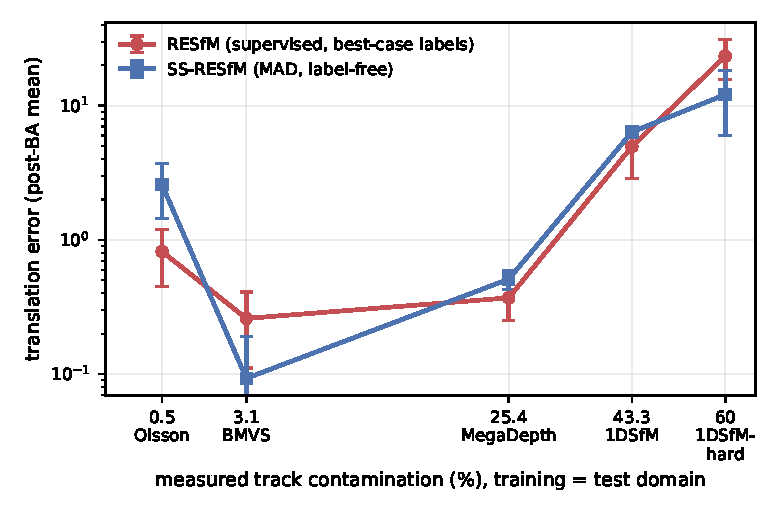
\includegraphics[width=0.88\textwidth]{fig_contamcurve.pdf}
\caption{\textbf{The in-distribution contamination curve.} Post-BA mean translation
(log scale) when training and test share the domain, versus measured contamination;
supervision uses best-case labels. Each label-free arm is its own line: soft weighting
($\pm$TTT) leads at low contamination, robust removal at high --- the mechanism flip,
replicated in-distribution. Supervision wins at $25\%$ and narrowly at $43\%$, is
seed-bimodal at $0.5\%$, and loses at $3.1\%$ (dead zone) and $60\%$ (label ceiling):
two distinct failure modes, not a smooth function of contamination. The rotation panel
makes the BlendedMVS dead zone starker ($20.7\pm12.2\deg$ vs.\ $4$--$13\deg$).
Bands: $\pm$std over five seeds.}
\label{fig:contamcurve}
\end{figure*}

\section{The same results through count- and coverage-based lenses}\label{app:lenses}
Our main tables follow the field's convention (RESfM, ESFM, GASFM): translation/rotation
means over each method's registered cameras, with $N_r$ reported alongside. That
convention answers ``how accurate is what you built'' but not ``how much of the scene
did you solve correctly,'' and it treats a dataset mean as the summary of a
distribution that, as the dtu106 decomposition shows, can be tail-dominated. This
appendix re-reads the complete five-seed matrix through three complementary lenses:
pairwise pose AUC with and without coverage pricing, per-scene win counts, and a
catastrophic-cell census. The lenses disagree with the means in instructive places;
we report all of them so no single convention carries a verdict alone.

\paragraph{Metrics and recovery.} For every (method, dataset, seed, scene) cell we
recover the final post-BA cameras from the saved COLMAP reconstructions, identify each
camera against the ground truth by its exact intrinsics (falling back to
track-coordinate voting where a scene shares intrinsics; identification $97$--$100\%$
per scene, validated against exact-intrinsics-unique cameras), and compute pairwise
relative-pose errors, which are invariant to each reconstruction's global similarity.
AUC@$30^{\circ}$ averages $(30-e)^{+}/30$ over registered pairs (pose error $e$ = max
of relative rotation angle and translation-direction angle); registration-aware
RA-AUC@$30^{\circ}$ averages over \emph{all} $\binom{N_c}{2}$ pairs, scoring pairs with
an unregistered camera at $180^{\circ}$ --- the coverage-priced convention of the
concurrent VGPA work~\cite{vgpa}.

\begin{table}[h]\centering\scriptsize
\setlength{\tabcolsep}{3pt}
\caption{\textbf{Pose AUC@$30^{\circ}$, five-seed mean$\pm$std.} Top block: RA-AUC
(coverage-priced). Bottom block: AUC over registered pairs only. Best per column in
bold. The two blocks disagree exactly where accuracy is bought with coverage.}
\label{tab:raauc}
\begin{tabular}{@{}lcccccc@{}}
\toprule
 & MegaDepth & 1DSfM & 1DSfM-hard & Strecha & BMVS & Olsson\\
\midrule
\multicolumn{7}{l}{\emph{RA-AUC@$30^{\circ}$ (all pairs; unregistered $=180^{\circ}$)}}\\[1pt]
\mad{}       & 0.599$\pm$0.02 & 0.374$\pm$0.01 & 0.067$\pm$0.01 & 0.587$\pm$0.03 & 0.589$\pm$0.07 & 0.568$\pm$0.01\\
weight       & 0.582$\pm$0.02 & 0.444$\pm$0.02 & 0.092$\pm$0.01 & 0.633$\pm$0.04 & 0.594$\pm$0.02 & 0.626$\pm$0.02\\
weight+TTT   & 0.580$\pm$0.02 & 0.445$\pm$0.02 & 0.092$\pm$0.01 & 0.635$\pm$0.03 & 0.595$\pm$0.02 & 0.627$\pm$0.03\\
remove       & 0.442$\pm$0.01 & 0.259$\pm$0.01 & 0.036$\pm$0.01 & 0.612$\pm$0.02 & 0.500$\pm$0.08 & 0.468$\pm$0.02\\
remove+TTT   & 0.442$\pm$0.01 & 0.262$\pm$0.01 & 0.037$\pm$0.01 & 0.609$\pm$0.02 & 0.501$\pm$0.08 & 0.467$\pm$0.02\\
hybrid       & 0.559$\pm$0.03 & 0.442$\pm$0.02 & 0.095$\pm$0.01 & 0.438$\pm$0.07 & 0.594$\pm$0.02 & 0.531$\pm$0.02\\
RESfM-scratch (sup.) & 0.605$\pm$0.01 & 0.408$\pm$0.01 & 0.044$\pm$0.01 & $\mathbf{0.725\pm0.08}$ & 0.600$\pm$0.01 & 0.620$\pm$0.01\\
ESFM (no mech.) & 0.574$\pm$0.02 & $\mathbf{0.461\pm0.01}$ & $\mathbf{0.099\pm0.01}$ & 0.662$\pm$0.03 & $\mathbf{0.722\pm0.06}$ & $\mathbf{0.645\pm0.01}$\\
ESFM$^{\ast}$ (clean tracks) & $\mathbf{0.691\pm0.04}$ & $\mathbf{0.461\pm0.02}$ & 0.035$\pm$0.01 & 0.517$\pm$0.03 & 0.652$\pm$0.10 & 0.570$\pm$0.14\\
\midrule
\multicolumn{7}{l}{\emph{AUC@$30^{\circ}$ (registered pairs only)}}\\[1pt]
\mad{}       & 0.778$\pm$0.02 & $\mathbf{0.642\pm0.03}$ & 0.354$\pm$0.06 & 0.601$\pm$0.03 & 0.642$\pm$0.08 & 0.640$\pm$0.02\\
weight       & 0.777$\pm$0.01 & 0.582$\pm$0.02 & 0.408$\pm$0.04 & 0.648$\pm$0.04 & 0.635$\pm$0.03 & 0.670$\pm$0.02\\
weight+TTT   & 0.777$\pm$0.01 & 0.578$\pm$0.02 & $\mathbf{0.411\pm0.03}$ & 0.650$\pm$0.04 & 0.637$\pm$0.03 & 0.674$\pm$0.02\\
remove       & 0.755$\pm$0.00 & 0.623$\pm$0.02 & $\mathbf{0.411\pm0.07}$ & 0.636$\pm$0.06 & 0.577$\pm$0.05 & 0.584$\pm$0.01\\
remove+TTT   & 0.748$\pm$0.00 & 0.638$\pm$0.02 & 0.388$\pm$0.03 & 0.634$\pm$0.06 & 0.578$\pm$0.05 & 0.581$\pm$0.02\\
hybrid       & 0.760$\pm$0.01 & 0.573$\pm$0.02 & 0.399$\pm$0.04 & 0.603$\pm$0.05 & 0.637$\pm$0.03 & 0.644$\pm$0.01\\
RESfM-scratch (sup.) & $\mathbf{0.811\pm0.01}$ & 0.623$\pm$0.03 & 0.329$\pm$0.06 & $\mathbf{0.735\pm0.07}$ & 0.654$\pm$0.02 & 0.653$\pm$0.02\\
ESFM (no mech.) & 0.756$\pm$0.01 & 0.570$\pm$0.01 & 0.409$\pm$0.04 & 0.677$\pm$0.05 & 0.744$\pm$0.05 & $\mathbf{0.688\pm0.01}$\\
ESFM$^{\ast}$ (clean tracks) & 0.790$\pm$0.05 & $\mathbf{0.669\pm0.04}$ & 0.330$\pm$0.07 & 0.519$\pm$0.03 & $\mathbf{0.760\pm0.06}$ & 0.607$\pm$0.15\\
\bottomrule
\end{tabular}
\end{table}

\begin{table}[h]\centering\scriptsize
\setlength{\tabcolsep}{3.5pt}
\caption{\textbf{Per-scene win counts vs.\ the supervised baseline} (matched-seed
scene$\times$seed cells, translation\,/\,rotation, as \% of cells), and the
catastrophic-cell census (cells with translation mean $>30$; in parentheses, cells
$>100$). The adaptive label-free arms have zero $>100$ cells anywhere; every $>100$
cell in the matrix is an Olsson/dtu106-family failure of an unrescued-trunk recipe.}
\label{tab:wincount}
\begin{tabular}{@{}lcccccc|ccc@{}}
\toprule
 & \multicolumn{6}{c|}{Win \% vs.\ supervised (trans/rot)} & \multicolumn{3}{c}{Cells $>30$ ($>100$)}\\
 & MD & 1DSfM & hard & Strecha & BMVS & Olsson & 1DSfM & hard & Olsson\\
\midrule
\mad{}       & 42/35 & 44/62 & 48/68 & 0/5   & 50/55 & 42/47 & 4/50 & 7/25 & 0/195\\
weight       & 31/24 & 36/58 & 48/56 & 15/40 & 55/55 & 45/50 & 6/50 & 8/25 & 0/195\\
weight+TTT   & 37/29 & 32/52 & 56/60 & 15/45 & 50/50 & 56/52 & 7/50 & 5/25 & 5/195 (5)\\
remove       & 41/34 & 66/78 & 80/84 & 0/0   & 30/50 & 39/42 & 5/50 & 2/25 & 0/195\\
remove+TTT   & 37/36 & 70/78 & 72/80 & 0/0   & 55/60 & 36/42 & 5/50 & 5/25 & 0/195\\
hybrid       & 37/32 & 30/54 & 48/68 & 0/0   & 55/50 & 44/47 & 9/50 & 8/25 & 0/194\\
RESfM-scratch (sup.) & --- & --- & --- & --- & --- & --- & 5/50 & 6/25 & 4/195 (4)\\
ESFM (no mech.) & 26/24 & 20/34 & 44/36 & 15/40 & 38/38 & 55/51 & 10/50 & 6/25 & 3/195 (3)\\
ESFM$^{\ast}$ (clean tracks) & 58/59 & 48/52 & 52/52 & 15/35 & 38/25 & 45/39 & 5/50 & 2/25 & 5/195 (5)\\
\bottomrule
\end{tabular}
\end{table}

\paragraph{The coverage-pricing inversion.} At $60\%$ contamination the two metric
families give opposite orderings. Plain remove --- the winner on translation means
($12.4\pm2.1$ vs.\ supervised $19.2\pm3.4$), medians, and win counts ($80/84\%$ of
cells) --- is \emph{last} under RA-AUC ($0.036$), because its $29\%$ registration
poisons over $90\%$ of camera pairs; the no-mechanism baseline, which loses every
raw-error comparison there, tops the RA column ($0.099$) by registering $40\%$.
AUC over registered pairs shows removal's accuracy is real (tied-best $0.411$): the
win is genuine \emph{on what it reconstructs}, and is bought with coverage. Neither
convention is ``the'' answer: raw error over registered cameras rewards aggressive
removal; coverage-priced AUC rewards registering more cameras at moderate error ---
the in-distribution analogue of the COLMAP registered-only caveat in our main table.
Every removal-family claim in this paper should be read with its $N_r$, and we
report both families so the reader can price coverage either way.

\paragraph{Counts, means, and tails disagree exactly where catastrophes live.}
ESFM$^{\ast}$ beats the supervised baseline on $58/59\%$ of MegaDepth cells while
losing the mean ($0.594$ vs.\ $0.365$, medians $0.071$ vs.\ $0.068$) --- clean tracks
are typically better per scene and blow up occasionally. Symmetrically, the supervised
baseline wins roughly half of the Olsson cells while losing the mean $2.5\times$, and
under RA-AUC@$30^{\circ}$ its Olsson score ($0.620$) sits \emph{above} \mad{}
($0.568$): a $30^{\circ}$-capped pairwise metric dilutes a single catastrophic scene
to its pair share, so the dtu106 failure that dominates the mean nearly vanishes from
the AUC. The win-count and AUC lenses are therefore not more honest than means ---
they are differently blind: means amplify tails, capped counts hide them. The
catastrophic-cell census (Table~\ref{tab:wincount}, right) is the tail-explicit
summary: across ${\sim}1{,}300$ scene$\times$seed cells, the adaptive label-free arms
produce \emph{zero} cells above $100$, while every unrescued-trunk recipe (supervised,
weight+TTT, no-mechanism, oracle-clean) produces them, all on Olsson. Reliability ---
the absence of catastrophic cells --- is the one verdict on which all lenses agree.

\paragraph{The contamination axis under coverage pricing.} Re-scoring the
in-distribution matrix (the main paper's in-distribution section) with RA-AUC@$30^{\circ}$ (five seeds
each): at $60\%$, supervision with best-case labels is \emph{last on both metric
families} --- worst-tier translation mean ($23.4\pm7.8$) and worst RA-AUC
($0.012\pm0.01$, from registering only ${\sim}106$ of $600$ cameras) --- so the
causal label-ceiling verdict, unlike the OOD removal ordering, is robust to how
coverage is priced (label-free soft arms lead at $0.088$--$0.090$). At low and
moderate contamination the no-mechanism baseline's coverage advantage makes it the
RA-AUC leader in-domain ($0.782/0.759/0.472$ at $0.5/3.1/43\%$, vs.\ supervised
$0.664\pm0.27$ --- the wide band is its in-domain bimodality); the mechanisms'
value under this lens, in distribution, is concentrated exactly where labels
fail.

\section{Per-scene results and configuration}\label{app:perscene}
\subsection{Per-scene results}\label{sec:perscene}
\begin{table*}[t]\centering\footnotesize
\caption{\textbf{Per-scene MegaDepth results} (layout follows RESfM's Table~1). For each
scene we show the number of input images ($N_c$) and the fraction of outlier
observations; for each model, the number of registered cameras ($N_r$) and mean
rotation ($e_R$, degrees) and translation ($e_t$) errors, post-BA, seed 20. Above the middle rule are Group~1
scenes ($<1000$ images); below are Group~2 scenes ($>1000$ images, subsampled to $300$
for testing), each group ordered by outlier fraction. Winning results per scene are
marked in bold and underlined. weight+TTT values are single draws of a run-to-run
nondeterministic evaluation (Sec.~\ref{sec:ttt}).}
\label{tab:supp_perscene_md}
\setlength{\tabcolsep}{2.5pt}%
\begin{tabular}{lrrrrrrrrrrrrrrr}
\toprule
& & & \multicolumn{3}{c}{madweight} & \multicolumn{3}{c}{weight} & \multicolumn{3}{c}{weight+TTT} & \multicolumn{3}{c}{RESfM}\\
\cmidrule(lr){4-6}\cmidrule(lr){7-9}\cmidrule(lr){10-12}\cmidrule(lr){13-15}
Scene & $N_c$ & \%out & $N_r$ & $e_R$ & $e_t$ & $N_r$ & $e_R$ & $e_t$ & $N_r$ & $e_R$ & $e_t$ & $N_r$ & $e_R$ & $e_t$\\
\midrule
0238 & 522 & 45\% & 437 & 19.02 & 1.41 & 137 & 8.23 & 0.62 & 141 & 8.37 & 0.63 & 355 & $\underline{\mathbf{1.40}}$ & $\underline{\mathbf{0.12}}$\\
0060 & 528 & 42\% & 469 & 0.29 & 0.03 & 476 & 0.20 & 0.02 & 452 & 4.13 & 0.37 & 494 & $\underline{\mathbf{0.04}}$ & $\underline{\mathbf{0.01}}$\\
0197 & 870 & 41\% & 470 & 7.22 & 0.89 & 341 & 3.54 & 0.38 & 422 & 6.94 & 1.11 & 739 & $\underline{\mathbf{0.97}}$ & $\underline{\mathbf{0.11}}$\\
0094 & 763 & 40\% & 493 & 2.72 & 0.45 & 505 & 1.44 & $\underline{\mathbf{0.16}}$ & 432 & $\underline{\mathbf{1.34}}$ & 0.17 & 572 & 5.33 & 0.88\\
0265 & 571 & 39\% & 457 & 17.62 & 3.26 & 477 & 5.78 & 2.34 & 547 & $\underline{\mathbf{0.60}}$ & $\underline{\mathbf{0.19}}$ & 424 & 16.27 & 3.09\\
0083 & 635 & 31\% & 342 & 4.34 & 0.23 & 511 & 17.70 & 1.56 & 317 & 3.20 & 0.20 & 582 & $\underline{\mathbf{1.40}}$ & $\underline{\mathbf{0.10}}$\\
0076 & 558 & 30\% & 423 & 1.40 & 0.38 & 519 & 0.61 & 0.23 & 454 & 0.74 & 0.22 & 499 & $\underline{\mathbf{0.25}}$ & $\underline{\mathbf{0.02}}$\\
0185 & 368 & 30\% & 347 & 0.21 & 0.01 & 335 & 0.24 & 0.04 & 321 & 0.88 & 0.09 & 352 & $\underline{\mathbf{0.07}}$ & $\underline{\mathbf{0.01}}$\\
0048 & 512 & 24\% & 475 & 1.93 & 0.14 & 467 & $\underline{\mathbf{0.35}}$ & $\underline{\mathbf{0.02}}$ & 450 & 0.43 & 0.03 & 489 & 1.85 & 0.11\\
0024 & 356 & 23\% & 299 & 1.27 & 0.18 & 291 & $\underline{\mathbf{1.13}}$ & $\underline{\mathbf{0.17}}$ & 289 & 4.78 & 1.13 & 334 & 3.67 & 1.09\\
0223 & 214 & 17\% & 205 & 2.66 & 0.24 & 198 & 1.69 & 0.23 & 199 & 3.06 & 0.30 & 204 & $\underline{\mathbf{0.45}}$ & $\underline{\mathbf{0.08}}$\\
5016 & 28 & 17\% & 23 & 0.27 & 0.04 & 25 & 0.08 & 0.02 & 28 & $\underline{\mathbf{0.07}}$ & 0.02 & 28 & 0.08 & $\underline{\mathbf{0.01}}$\\
0046 & 440 & 15\% & 422 & $\underline{\mathbf{2.88}}$ & $\underline{\mathbf{0.22}}$ & 421 & 4.11 & 0.30 & 419 & 3.88 & 0.25 & 410 & 14.64 & 0.93\\
\midrule
0099 & 299 & 47\% & 224 & $\underline{\mathbf{0.81}}$ & 0.15 & 216 & 2.77 & 3.52 & 212 & 1.58 & $\underline{\mathbf{0.13}}$ & 252 & 2.18 & 0.39\\
1001 & 285 & 44\% & 280 & 1.58 & 1.22 & 278 & 1.49 & 0.73 & 279 & $\underline{\mathbf{1.22}}$ & $\underline{\mathbf{0.49}}$ & 273 & 1.23 & 0.50\\
0231 & 296 & 42\% & 274 & 1.63 & 0.15 & 257 & 0.64 & 0.07 & 264 & 1.49 & 0.24 & 265 & $\underline{\mathbf{0.17}}$ & $\underline{\mathbf{0.02}}$\\
0411 & 299 & 30\% & 281 & 0.22 & 0.03 & 245 & 2.99 & 0.32 & 250 & 4.12 & 0.46 & 275 & $\underline{\mathbf{0.11}}$ & $\underline{\mathbf{0.02}}$\\
0377 & 295 & 28\% & 200 & 0.62 & 0.05 & 222 & 2.76 & 0.26 & 243 & $\underline{\mathbf{0.56}}$ & $\underline{\mathbf{0.03}}$ & 223 & 0.82 & 0.06\\
0102 & 299 & 26\% & 289 & 0.15 & 0.02 & 289 & $\underline{\mathbf{0.07}}$ & $\underline{\mathbf{0.01}}$ & 291 & 0.08 & 0.01 & 287 & 0.10 & 0.02\\
0147 & 298 & 25\% & 261 & 31.69 & 2.99 & 235 & 15.28 & 1.21 & 225 & 15.27 & $\underline{\mathbf{1.20}}$ & 247 & $\underline{\mathbf{4.61}}$ & 3.22\\
0148 & 287 & 25\% & 220 & 2.60 & 0.33 & 201 & 2.11 & 0.11 & 196 & $\underline{\mathbf{0.62}}$ & 0.04 & 202 & 0.94 & $\underline{\mathbf{0.04}}$\\
0446 & 298 & 22\% & 292 & $\underline{\mathbf{0.40}}$ & $\underline{\mathbf{0.03}}$ & 285 & 1.20 & 0.19 & 292 & 1.04 & 0.19 & 293 & 0.71 & 0.05\\
0022 & 297 & 21\% & 275 & 0.14 & 0.02 & 272 & 0.22 & 0.03 & 267 & 0.33 & 0.04 & 276 & $\underline{\mathbf{0.11}}$ & $\underline{\mathbf{0.02}}$\\
0327 & 298 & 21\% & 282 & 1.97 & 0.09 & 285 & 0.22 & 0.02 & 284 & 0.21 & 0.02 & 277 & $\underline{\mathbf{0.09}}$ & $\underline{\mathbf{0.01}}$\\
0015 & 284 & 21\% & 196 & 2.64 & 0.30 & 196 & 3.87 & 0.56 & 211 & 3.90 & 0.65 & 232 & $\underline{\mathbf{1.31}}$ & $\underline{\mathbf{0.30}}$\\
0455 & 298 & 20\% & 283 & $\underline{\mathbf{0.20}}$ & $\underline{\mathbf{0.01}}$ & 285 & 0.21 & 0.01 & 288 & 0.46 & 1.60 & 293 & 0.85 & 0.09\\
0496 & 297 & 19\% & 279 & $\underline{\mathbf{0.27}}$ & 0.04 & 285 & 0.50 & $\underline{\mathbf{0.04}}$ & 287 & 1.28 & 0.09 & 283 & 0.46 & 0.07\\
1589 & 299 & 17\% & 265 & 0.96 & 0.06 & 262 & 0.28 & 0.05 & 296 & 1.91 & 0.30 & 291 & $\underline{\mathbf{0.06}}$ & $\underline{\mathbf{0.01}}$\\
0012 & 299 & 16\% & 281 & $\underline{\mathbf{0.23}}$ & $\underline{\mathbf{0.02}}$ & 247 & 9.51 & 0.70 & 262 & 2.76 & 0.22 & 288 & 5.53 & 0.34\\
0104 & 284 & 16\% & 189 & 0.32 & 0.03 & 193 & 2.28 & 0.18 & 194 & 1.44 & 0.07 & 199 & $\underline{\mathbf{0.30}}$ & $\underline{\mathbf{0.02}}$\\
0019 & 299 & 15\% & 232 & 3.22 & 0.17 & 253 & 6.55 & 0.28 & 264 & 3.24 & 0.13 & 252 & $\underline{\mathbf{0.05}}$ & $\underline{\mathbf{0.01}}$\\
0063 & 293 & 14\% & 258 & 0.63 & 0.08 & 268 & 0.72 & 0.07 & 267 & 0.65 & $\underline{\mathbf{0.06}}$ & 266 & $\underline{\mathbf{0.44}}$ & 0.07\\
0130 & 285 & 14\% & 250 & 10.17 & 1.60 & 184 & 1.87 & 0.16 & 185 & $\underline{\mathbf{0.33}}$ & $\underline{\mathbf{0.01}}$ & 195 & 1.03 & 0.07\\
0080 & 284 & 13\% & 132 & 1.10 & $\underline{\mathbf{0.05}}$ & 148 & 2.48 & 0.20 & 147 & 0.70 & 0.07 & 141 & $\underline{\mathbf{0.66}}$ & 0.10\\
0240 & 298 & 12\% & 275 & $\underline{\mathbf{2.23}}$ & $\underline{\mathbf{0.25}}$ & 275 & 4.64 & 0.34 & 272 & 5.32 & 0.46 & 282 & 3.02 & 0.35\\
0007 & 290 & 12\% & 106 & $\underline{\mathbf{0.07}}$ & $\underline{\mathbf{0.01}}$ & 269 & 1.86 & 0.09 & 261 & 3.28 & 0.14 & 104 & 0.99 & 0.04\\
\bottomrule
\end{tabular}
\end{table*}

\begin{table*}[t]\centering\footnotesize
\caption{\textbf{Per-scene 1DSfM results} (layout follows RESfM's Table~1). Columns as in
Table~\ref{tab:supp_perscene_md}; seed 20, scenes ordered by outlier fraction. Winning results per scene are marked in bold and
underlined.}
\label{tab:supp_perscene_1dsfm}
\setlength{\tabcolsep}{2.5pt}%
\begin{tabular}{lrrrrrrrrrrrrrrr}
\toprule
& & & \multicolumn{3}{c}{madweight} & \multicolumn{3}{c}{weight} & \multicolumn{3}{c}{weight+TTT} & \multicolumn{3}{c}{RESfM}\\
\cmidrule(lr){4-6}\cmidrule(lr){7-9}\cmidrule(lr){10-12}\cmidrule(lr){13-15}
Scene & $N_c$ & \%out & $N_r$ & $e_R$ & $e_t$ & $N_r$ & $e_R$ & $e_t$ & $N_r$ & $e_R$ & $e_t$ & $N_r$ & $e_R$ & $e_t$\\
\midrule
Ellis\_Island & 227 & 56\% & 180 & $\underline{\mathbf{17.16}}$ & 17.59 & 171 & 17.37 & $\underline{\mathbf{15.90}}$ & 177 & 17.74 & 17.11 & 192 & 18.15 & 16.02\\
NYC\_Library & 332 & 54\% & 282 & 2.32 & 2.94 & 261 & $\underline{\mathbf{1.16}}$ & $\underline{\mathbf{1.19}}$ & 279 & 10.30 & 3.39 & 285 & 12.99 & 6.28\\
Vienna\_Cathedral & 836 & 51\% & 537 & 7.42 & 7.30 & 484 & $\underline{\mathbf{0.46}}$ & 22.71 & 651 & 26.80 & 33.57 & 492 & 1.09 & $\underline{\mathbf{2.29}}$\\
Notre\_Dame & 553 & 48\% & 507 & 3.33 & 0.68 & 491 & 1.00 & 0.34 & 485 & $\underline{\mathbf{0.83}}$ & $\underline{\mathbf{0.33}}$ & 493 & 1.08 & 0.49\\
Yorkminster & 437 & 45\% & 299 & 8.05 & $\underline{\mathbf{5.79}}$ & 371 & 14.95 & 30.87 & 380 & 12.20 & 10.79 & 309 & $\underline{\mathbf{6.88}}$ & 8.77\\
Piazza\_del\_Popolo & 338 & 42\% & 218 & $\underline{\mathbf{0.43}}$ & $\underline{\mathbf{0.94}}$ & 265 & 19.54 & 10.66 & 254 & 20.46 & 17.05 & 255 & 3.15 & 2.49\\
Tower\_of\_London & 472 & 42\% & 317 & 35.61 & 76.34 & 337 & 23.30 & $\underline{\mathbf{28.29}}$ & 314 & $\underline{\mathbf{17.91}}$ & 72.61 & 299 & 49.66 & 67.95\\
Montreal\_Notre\_Dame & 450 & 36\% & 311 & 0.59 & 0.94 & 325 & $\underline{\mathbf{0.55}}$ & 11.35 & 320 & 0.81 & 1.24 & 400 & 0.59 & $\underline{\mathbf{0.93}}$\\
Alamo & 577 & 29\% & 467 & 2.45 & 1.77 & 507 & 2.74 & 2.18 & 497 & 2.49 & $\underline{\mathbf{1.67}}$ & 502 & $\underline{\mathbf{2.42}}$ & 1.73\\
Madrid\_Metropolis & 341 & 29\% & 249 & 5.72 & 9.63 & 301 & 2.84 & 4.37 & 295 & 2.35 & 3.52 & 287 & $\underline{\mathbf{1.82}}$ & $\underline{\mathbf{3.38}}$\\
\bottomrule
\end{tabular}
\end{table*}

Tables~\ref{tab:supp_perscene_md} and~\ref{tab:supp_perscene_1dsfm} report the per-scene
post-BA translation and rotation errors and registered-camera counts underlying the
main paper's dataset-level numbers (seed 20, the declared pipeline): the 36 MegaDepth test scenes and the ten 1DSfM
scenes, for the three self-supervised arms (madweight, weight, weight+TTT) and the
supervised RESfM baseline trained from scratch under the identical
recipe. The per-scene view makes two aggregate statements concrete: on 1DSfM no single
arm dominates, the best mechanism flips scene by scene (with Ellis\_Island and
Tower\_of\_London hard for every arm), consistent with the per-scene complementarity
analysis in the main paper; on MegaDepth the four arms are close on most scenes and the
dataset-level gap is dominated by a handful of high-error scenes. Per scene, the
catastrophic scenes (Ellis\_Island, Tower\_of\_London) fail in both metrics, though
rotation does not always track translation (weight's Vienna\_Cathedral failure is
translation-specific: $22.71/0.46$), and $N_r$ stays in the $58$--$92\%$ range of each scene's images on 1DSfM
with no arm systematically dropping scenes.
The dataset-level rotation and registration record accompanies the main comparison (Table~2 of the main paper). Rotation broadly agrees with translation
at the dataset level: the supervised BlendedMVS failure is even larger in rotation
($36\deg$) and the high-contamination ordering is preserved, though the best arm can
differ per metric (on MegaDepth, weight+TTT leads translation while RESfM leads
rotation). Registration is contamination-dependent: the supervised baseline registers
the most cameras in distribution ($85\%$ vs.\ $78$--$80\%$ on MegaDepth) and on clean
Strecha, while under high contamination the label-free arms retain more cameras than
supervision ($38$--$43\%$ vs.\ $37\%$ on 1DSfM-hard) at lower error (madweight).
















\begin{table}[tb]\centering\footnotesize
\caption{\textbf{Training and evaluation configuration.} All arms in the main paper use
these settings; the only per-method difference is the base learning rate.}
\label{tab:supp_config}
\setlength{\tabcolsep}{4pt}%
\begin{tabular}{ll}
\toprule
Setting & Value\\
\midrule
\multicolumn{2}{l}{\emph{Training (both methods)}}\\
Epochs & 20{,}000 (one epoch = one pass over all scenes)\\
Batch & 4 scenes\\
LR schedule & milestones $10\text{k},11\text{k},\ldots,20\text{k}$, $\gamma=0.9$\\
Base LR & $10^{-4}$ (SS-RESfM) / $10^{-3}$ (RESfM)\\
Loss weights & $\alpha_{\text{reproj}}=1$, $\beta_{\text{cls}}=1$\\
Infinity-point margin & $10^{-4}$\\
Checkpoint selection & best validation error, evaluated every 500 epochs\\
Seed & 20 (21--22 / 21--24 for the seed studies)\\
\midrule
\multicolumn{2}{l}{\emph{Adaptive pseudo-labels (SS-RESfM only)}}\\
Inlier / outlier percentile & 20 / 80 (of per-observation reproj.\ error)\\
Threshold separation & scale-aware floor, $0.25\times$ median error\\
Warm-up & 10 epochs before pseudo-labeling starts\\
\midrule
\multicolumn{2}{l}{\emph{Evaluation}}\\
Removal threshold $\tau$ & 0.6 (0.8 for low-contamination single-\\
 & camera sets, following RESfM)\\
Test-time fine-tuning & 1{,}001 iterations, LR $5\times10^{-3}$,\\
 & evaluated every 250 iterations\\
Bundle adjustment & pyceres/pycolmap robust BA, as RESfM\\
\bottomrule
\end{tabular}
\end{table}

\section{Comparison with ESFM in both of its regimes}\label{app:esfmboth}
ESFM is the no-outlier-mechanism ancestor of this model family and operates in two
regimes: multi-scene training and its original per-scene optimization. We compare in
both.

\paragraph{Multi-scene (same contaminated tracks).} Vanilla ESFM --- the ESFM
architecture inside the RESfM codebase, so trainer, tracks, and BA are identical to
every other arm --- trained under the unified protocol (reference row in the main
table; five-seed bands) reaches
$0.71\pm0.11$ on MegaDepth, $18.42\pm0.75$ on 1DSfM, $21.76\pm0.80$ at $60\%$,
$2.03\pm0.14$ on Strecha, $6.45\pm3.75$ on BlendedMVS, and $5.91\pm3.32$ on Olsson.
Three readings. First, without any outlier mechanism, contaminated training data
degrades every contaminated benchmark relative to all mechanism-equipped arms --- the
premise of RESfM and of this paper. Second, its apparent BlendedMVS competitiveness at
seed $20$ ($0.23$) dissolves at five seeds ($6.45\pm3.75$, bimodal) --- one more
single-seed verdict reversed by banding (cf.\ the seed-additivity analysis) --- and
its Olsson behaviour is likewise bimodal (collapse in three of five seeds), so the
clean-OOD failure mode predates the supervised head and lives in the trunk. Third, on
Strecha the band ($2.03\pm0.14$) statistically ties the best label-free soft arms
($1.97$--$2.00$), confirming at band level that at the clean extreme the correct
mechanism approaches none.

\paragraph{Single-scene (ESFM's original per-scene optimization, Olsson).} Here the
primary ESFM row runs in the \emph{authors' official ESFM codebase}; the RESfM-codebase
reimplementation is included as a cross-check and agrees to within noise ($0.19$ vs.\
$0.22\deg$), ruling out implementation gaps between the two regimes. On $36$ calibrated
Olsson scenes ($3$ runs each, matching ESFM's protocol), post-BA median-over-scenes
rotation/translation:
\begin{center}\footnotesize
\begin{tabular}{lcc}
\toprule
Method (per-scene optimization) & Rot ($\deg$) & Trans\\
\midrule
ESFM (official code)            & 0.19 & 0.057\\
ESFM (RESfM codebase)           & 0.22 & 0.088\\
ESFM $+$ sequential init ($10$ scenes) & 0.10 & 0.032\\
ESFM $+$ MAD statistic          & 0.68 & 0.123\\
self-supervised arm (base)      & 8.03 & 0.748\\
self-supervised arm (30/70 percentiles) & 2.81 & 0.434\\
self-supervised arm $+$ TTT     & 1.22 & 0.324\\
\bottomrule
\end{tabular}
\end{center}
Vanilla ESFM wins this regime outright, and every outlier mechanism --- statistical or
learned --- costs accuracy. This is not a failure of the mechanisms but the
low-contamination end of the complementarity finding replicated in a second regime: at
$0.5\%$ contamination with per-scene optimization there is nothing to reject, and any
removal or reweighting machinery only discards signal. The practical reading matches
the main paper: mechanism choice must adapt to contamination, and ``none'' is the
correct mechanism at the clean extreme of the axis.


\section{Alternative designs we tested}\label{app:altdesigns}
The complementarity finding says the best outlier mechanism depends on contamination,
which invites an obvious question: can a better \emph{design} remove the dependence?
We tested eleven alternatives spanning the loss, the head, the input representation and
the supervision signal, each trained with the same recipe, tracks and schedule as the
arms it is compared against, on the $43\%$-contamination in-distribution pool
(\S\ref{sec:indist}), with \textbf{five training seeds each} ($44$ trainings).

\begin{table}[h]\centering\footnotesize
\caption{\textbf{Alternative designs}, post-BA translation on the held-out test scenes of
the $43\%$ pool, mean$\pm$std over five training seeds, sorted by mean. ``Base'' is the
recipe each variant modifies, and therefore the control it must beat: supervised
$4.97\pm2.08$, self-supervised \mad{} $6.37\pm0.20$. The last column is the seed-$20$
value alone --- what a single-run screen would have reported.}
\label{tab:altdesigns}
\setlength{\tabcolsep}{4pt}%
\begin{tabular}{llccc}
\toprule
Variant & Base & mean$\pm$std & range & seed $20$ only\\
\midrule
GT$+$SS loss, $0.25/0.75$ & supervised & 5.59$\pm$0.51 & 5.03--6.03 & 5.04\\
GT$+$SS loss, $0.50/0.50$ & supervised & 5.80$\pm$0.64 & 5.20--6.75 & 6.17\\
GT$+$SS loss, $0.75/0.25$ & supervised & 5.83$\pm$0.59 & 5.15--6.75 & 5.15\\
unrolled IRLS refinement & self-supervised & 6.58$\pm$0.47 & 5.93--7.19 & 6.43\\
SS$+$GT loss, $0.25/0.75$ & self-supervised & 6.73$\pm$0.33 & 6.39--7.16 & 6.76\\
soft pseudo-labels ($\tau{=}1$) & self-supervised & 6.78$\pm$0.37 & 6.23--7.20 & 6.72\\
soft pseudo-labels ($\tau{=}2$) & self-supervised & 6.89$\pm$0.23 & 6.55--7.09 & 7.09\\
learned robust loss (Cauchy NLL) & self-supervised & 6.98$\pm$1.70 & 5.90--9.97 & 6.13\\
SS$+$GT loss, $0.75/0.25$ & self-supervised & 7.68$\pm$1.62 & 6.60--10.48 & 6.66\\
track-statistic input channels & self-supervised & 7.73$\pm$1.75 & 6.46--10.77 & 7.56\\
SS$+$GT loss, $0.50/0.50$ & self-supervised & 7.75$\pm$1.68 & 6.43--10.48 & 10.48\\
\bottomrule
\end{tabular}
\end{table}

\paragraph{What the variants are.} \emph{GT$+$SS loss} adds the self-supervised
confident-pseudo-label term to the supervised classification loss (and vice versa for
\emph{SS$+$GT}), splitting the same classification budget in the stated ratio, so the
variant differs from its base only in \emph{which} targets the classification term
follows. \emph{Learned robust loss} replaces the score-weighted reprojection term with a
Cauchy negative log-likelihood $\log s + \log(1+(r/s)^2)$ over a per-observation scale
$s$ emitted by a second head channel: soft weighting and removal become two limits of
one \emph{learned} mechanism rather than a choice made per dataset. \emph{Unrolled IRLS}
recomputes residuals from the current prediction, converts them to Cauchy weights and
re-runs the blocks, folding the robust re-estimation that bundle adjustment performs
afterwards into the network. \emph{Track-statistic channels} append eight label-free
geometric features per observation (track length, camera degree, co-visibility of the
supporting cameras, coordinate spread). \emph{Soft pseudo-labels} replace the hard
$0/1$ confident-band target with a continuous ramp across the band, removing the
unlabelled dead zone.

\paragraph{None improves on its base.} The three supervised-side dual-loss variants land
\emph{inside} the supervised band ($5.59$--$5.83$ vs.\ $4.97\pm2.08$): mixing a
self-supervised term into label supervision is neutral, neither the rescue one might
hope for at $43\%$ contamination nor a harm. Every self-supervised-side variant is worse
than plain \mad{} ($6.37\pm0.20$), including the two that are conceptually most
appealing --- the learned robust loss ($6.98\pm1.70$) and unrolled IRLS
($6.58\pm0.47$). The design space around this architecture is, in our hands, flat.

\paragraph{Single-seed screens would have reported four of these wrong.} Each variant
was first run at seed $20$ only, as a screen. Comparing that column with the bands,
\textbf{four of eleven screens invert}: the learned robust loss scored $6.13$ at seed
$20$ --- below \emph{every} seed of its control --- yet bands at $6.98\pm1.70$; the
SS-side $0.50/0.50$ variant scored $10.48$, its \emph{worst} seed, and bands at
$7.75\pm1.68$; the SS-side $0.75/0.25$ variant scored its \emph{best} seed; and the
supervised $0.50/0.50$ variant read as a clear loss at $6.17$ but bands inside the
control at $5.80\pm0.64$. The four variants with the widest bands ($\pm1.6$--$1.75$) are
exactly the four whose screens misled. This is the paper's seed-reliability argument
turned on our own experiments: in this family a single-run architecture comparison is
not evidence, in either direction.

\paragraph{Scope.} These are single-pool results ($43\%$ contamination, three held-out
test scenes, fixed evaluation seed). A variant that fails here could still help at a
different contamination level, and we did not extend the grid; what the table supports
is the narrower claim that none of these designs is a drop-in improvement where we
tested it.

\section{Cross-generalization: every training domain, every test domain}\label{app:crossgen}
We train both recipes on each of the six domains (in-distribution protocol of
the main paper's in-distribution study: GT-derived labels for the supervised arm) and evaluate every model
on \emph{all} datasets ($\sim$5{,}400 evaluations; five training seeds per cell,
strechaid two). Cells where a pool's training scenes overlap the target are excluded.
Table~\ref{tab:crossgen} reports \mad{}\,/\,supervised post-BA translation means.

\begin{table*}[t]\centering\footnotesize
\caption{\textbf{Cross-generalization grid}: rows = training domain, columns = test
dataset; each cell \mad{}\,/\,supervised (mean$\pm$std over training seeds). Diagonal
(*) = held-out in-distribution test (Table~4 of the main paper); ``leak'' = training
scenes overlap the target.}
\label{tab:crossgen}
\setlength{\tabcolsep}{2.5pt}%
\resizebox{\textwidth}{!}{%
\begin{tabular}{lcccccc}
\toprule
Trained on $\downarrow$ & MegaDepth & Olsson & Strecha & BMVS & 1DSfM & 1DSfM-hard\\
\midrule
Olsson & 0.52\,/\,0.62 & *1.97\,/\,2.03 & 3.05\,/\,\textbf{0.72} & 6.97\,/\,6.70 & 11.84\,/\,12.04 & \textbf{15.56}\,/\,20.17\\
Strecha (2 seeds) & 0.53\,/\,0.54 & \textbf{2.69}\,/\,8.62 & *0.01\,/\,0.01 & 7.29\,/\,8.08 & 13.94\,/\,\textbf{10.22} & 17.06\,/\,18.97\\
BMVS & 0.63\,/\,0.51 & \textbf{2.73}\,/\,6.95 & 2.56\,/\,\textbf{1.44} & *0.09\,/\,0.26 & 11.50\,/\,10.45 & 19.70\,/\,18.59\\
1DSfM-easy & 0.53\,/\,0.56 & \textbf{3.27}\,/\,7.20 & 2.94\,/\,\textbf{1.92} & 6.48\,/\,5.81 & *6.37\,/\,4.97 & \textbf{18.31}\,/\,20.12\\
1DSfM-hard & 0.47\,/\,0.83 & \textbf{2.93}\,/\,7.78 & 3.02\,/\,\textbf{1.94} & 3.65\,/\,5.68 & 13.21\,/\,\textbf{8.49} & *12.1\,/\,23.4\\
1DSfM-merged & 0.52\,/\,0.59 & \textbf{3.34}\,/\,4.96 & 2.98\,/\,\textbf{2.37} & 7.26\,/\,6.69 & *6.71\,/\,5.05 & leak\\
\bottomrule
\end{tabular}}
\end{table*}

Three findings generalize beyond MegaDepth training. \emph{(i) The clean-benchmark
collapse is training-domain-invariant --- and so is its tail structure}: the
supervised recipe degrades on Olsson OOD from \emph{every} training domain
($4.96$--$8.62$ across five pools, seed-volatile up to $\pm4.25$), while \mad{} lands
in a tight $2.69$--$3.34$ band from every pool. The tail decomposition of the main
paper holds pool-by-pool: the supervised dtu106 catastrophic failure fires from every
training domain (on $1$--$5$ of $5$ seeds per pool, errors ${\sim}230$--$360$ vs.\
${\sim}1$ on the escaping seeds --- a pure basin lottery), whereas \mad{} stays at
${\le}7$ on that scene in all $27$ cells; excluding dtu106, a modest supervised
deficit persists in four of five pools ($3.4$--$4.3$ vs.\ $2.7$--$3.3$). The
reliability asymmetry --- both the lottery and the residual gap --- is a property of
the recipes, not of MegaDepth. \emph{(ii)
The Strecha exception is likewise invariant}: supervision wins Strecha from every
training domain ($0.72$--$2.37$ vs.\ $2.56$--$3.05$). \emph{(iii) At the extreme
($60\%$ target), \mad{} from any domain beats supervision from any domain} (best
supervised cell $18.59$ vs.\ \mad{} $15.56$--$19.70$, with the in-distribution
\mad{} at $12.1$) --- and, remarkably, MegaDepth as a \emph{test} set is nearly
training-domain-independent (all cells $0.47$--$0.83$), suggesting its curated test
scenes are easy for any reasonably trained model of this family. One
counterexample sharpens the picture: supervised trained on 1DSfM-hard generalizes to
standard 1DSfM \emph{better} than anything else ($8.49$), consistent with supervision
learning transferable contamination statistics when its labels are sound on a related
domain.

\section{Per-scene label degradation}\label{app:labeldeg}
Table~\ref{tab:supp_labelceiling} gives the per-scene data behind the main paper's
label-ceiling analysis: for each of the 18 scenes we measure the contamination level, the
fraction of track observations that receive a COLMAP-derived label at all (coverage), and
the precision and recall of those labels against ground truth. The aggregate trend in the main paper is visible scene by scene: below ${\sim}10\%$ contamination coverage is $0.92$--$1.00$ and recall is $0.66$--$0.97$ (mostly above $0.8$), while above ${\sim}15\%$ contamination recall never exceeds $0.50$ on any scene ($0.25$--$0.50$) and coverage falls as low as $0.37$: the supervision signal degrades exactly where outlier handling matters most.




\begin{table}[t]\centering\footnotesize
\caption{\textbf{Per-scene label-degradation results.} For each scene: contamination (fraction of track observations that are GT outliers), COLMAP-label coverage (fraction of observations receiving a label), and precision/recall of the COLMAP-derived outlier labels against GT, sorted by contamination. Above ${\sim}15\%$ contamination, label recall never exceeds $0.50$: the labels miss at least half of the true outliers.}
\label{tab:supp_labelceiling}
\setlength{\tabcolsep}{3.5pt}%
\begin{tabular}{llcccc}
\toprule
Dataset & Scene & Contam.\ (\%) & Coverage & Prec. & Recall\\
\midrule
BlendedMVS & 58c4bb4f4a\ldots & 0.5 & 1.00 & 0.86 & 0.94\\
Strecha & Herz-Jesu-P8 & 0.7 & 1.00 & 0.51 & 0.66\\
Strecha & fountain-P11 & 0.7 & 1.00 & 0.69 & 0.76\\
Strecha & Herz-Jesu-P25 & 2.6 & 0.99 & 0.72 & 0.82\\
Strecha & entry-P10 & 2.7 & 0.99 & 0.88 & 0.88\\
BlendedMVS & 5be883a4f9\ldots & 4.0 & 0.98 & 0.90 & 0.84\\
BlendedMVS & 5b6e716d67\ldots & 6.1 & 0.92 & 0.89 & 0.92\\
BlendedMVS & 5bfd0f32ec\ldots & 7.1 & 0.97 & 0.97 & 0.97\\
BlendedMVS & 5b950c7160\ldots & 9.2 & 0.96 & 0.92 & 0.94\\
MegaDepth & 0007 & 11.2 & 0.73 & 0.84 & 0.47\\
1DSfM & Alamo & 26.6 & 0.76 & 0.81 & 0.25\\
1DSfM & Madrid\_Metropolis & 28.8 & 0.67 & 0.85 & 0.28\\
MegaDepth & 0041 & 31.4 & 0.49 & 0.80 & 0.42\\
MegaDepth & 0060 & 39.0 & 0.42 & 0.53 & 0.45\\
1DSfM & Piazza\_del\_Popolo & 41.9 & 0.76 & 0.90 & 0.30\\
MegaDepth & 0047 & 54.9 & 0.37 & 0.83 & 0.50\\
1DSfM & Ellis\_Island & 57.9 & 0.79 & 0.89 & 0.37\\
1DSfM-hard & Gendarmenmarkt & 59.8 & 0.50 & 0.89 & 0.29\\
\bottomrule
\end{tabular}
\end{table}


\section{Pre- versus post-BA seed variability}\label{app:prepost}
Table~\ref{tab:prepost} reports, for every arm and dataset, the five-seed band of the
\emph{network} output (pre-BA) next to the band after robust bundle adjustment. The
behaviour is what one expects of a non-linear optimiser with multiple basins, and it is
worth recording because two statements in the main text depend on it.

A direct control separates the two sources. Re-evaluating the authors' \emph{fixed}
released weights under five evaluation seeds gives $0.203\pm0.008$ on MegaDepth
(pre-BA $1.730\pm0.005$), $10.71\pm0.27$ on 1DSfM, and \emph{identical} values to two
decimals on Strecha ($0.20$) and BlendedMVS ($0.33$): with the network held constant,
bundle adjustment is close to deterministic, and exactly deterministic on the small
clean sets. The large bands below therefore reflect genuine differences between
independently trained networks, amplified by BA, and not evaluation noise. A full
paired-seed replication confirms this at scale: re-running all $2{,}352$ evaluations with
the evaluation seed set equal to each cell's training seed (rather than fixed at $20$)
reproduces every five-seed band within a fraction of its std --- e.g.\ the baseline row
moves from $0.37\pm0.12$ to $0.38\pm0.14$ on MegaDepth and is unchanged to two decimals
on Strecha, BlendedMVS, and Olsson --- with the largest shifts in the TTT cells
($\sim\!0.13$), consistent with their run-to-run nondeterminism. The choice of
evaluation seed is immaterial to every conclusion in this paper.

First, on the contaminated datasets nearly all seed variability is created by bundle
adjustment, not by training: pre-BA bands are $\pm0.02$--$0.13$ for the self-supervised
arms and $\pm0.05$--$0.43$ for the baseline (relative spreads of ${\sim}0.5\%$ and
$1$--$3\%$ respectively), while the same cells after BA carry $\pm1.7$--$4.1$. The
networks are highly reproducible across seeds; most of the pipeline's variance enters at
the BA stage, which lowers the error on $234$ of $242$ baseline scene evaluations we
examined while widening the \emph{relative} seed band by an order of magnitude --- BA
compresses the mean and amplifies the spread. This is the seed-level counterpart of the
environment-level chaotic basin selection documented in App.~\ref{app:repro}, now
measured over $36$ independent cells.

Second, the removal arms do not produce better raw geometry than supervision --- they
produce geometry that robust BA can repair. Pre-BA the supervised baseline leads
everywhere (MegaDepth $1.76$ vs.\ ${\sim}3.03$; 1DSfM $22.1$ vs.\ $25.3$--$26.6$), yet
plain removal improves by $2.9\times$ through BA at $60\%$ contamination
($36.3\to12.4$) against the baseline's $1.9\times$ ($35.8\to19.2$), and by $5.0\times$
on Olsson ($17.1\to3.4$) against $1.5\times$ ($11.0\to7.4$). Feeding BA a cleaner
observation set, rather than a more accurate initialisation, is the mechanism behind the
high-contamination result.

A third observation concerns the baseline specifically, and is the one exception to the
first: its clean-OOD instability is already present \emph{before} BA (Strecha
$0.68\pm0.78$, Olsson $11.01\pm2.27$, versus $\pm0.18$--$0.24$ and $\pm0.19$--$0.47$ for
the self-supervised arms), locating that failure in supervised training rather than in
bundle adjustment or evaluation. Per scene the failure is bimodal and seed-contingent
rather than noisy: entry-P10 costs $0.04$--$0.06$ on three seeds and $4.0$/$7.0$ on the
other two; dtu106 sits at $250$--$260$ on four seeds and $53$ on one. Five
authors-faithful retrains (seeds $20$--$24$, the authors' validation metric and margin)
reproduce the scratch baseline's band on every dataset --- including the
one-bad-Strecha-seed pattern and the four-of-five Olsson collapse ($8.66$--$9.02$ with a
single $2.32$ escape, mirroring the scratch $2.69$) --- so these failure modes belong to
the supervised recipe,  not to our retraining of it.

\paragraph{The two checkpoint-selection rules are statistically indistinguishable.}
Both rules ran the same five seeds, so they admit a paired comparison. On MegaDepth the
authors' Accuracy-based selection gives $[0.496, 0.260, 0.300, 0.310, 0.223]$ (mean
$0.318\pm0.106$) and our label-free reprojection-based selection $[0.344, 0.189, 0.423,
0.529, 0.340]$ ($0.365\pm0.125$); per-seed differences $[-0.152, -0.071, +0.123,
+0.219, +0.117]$, paired mean $+0.047\pm0.153$, $t(4)=0.69$ (vs.\ $2.78$ for
$p<0.05$). Our rule wins two of five seeds. The single-run pair in the reference rows
($0.496$ vs.\ $0.37$) is seed $20$, the most extreme of the five and the one most
favourable to our rule --- hence we claim only that the deviation does not advantage
us.

\begin{table}[h]\centering\footnotesize
\caption{\textbf{Checkpoint selection, all six datasets}: from-scratch RESfM under our
label-free reprojection rule vs.\ the authors' Accuracy rule (identical recipe, identical
tracks, same five seeds). Paired $t(4)$ needs $|t|>2.78$ for $p<0.05$; no dataset
approaches it, and the sign of the difference flips across datasets.}
\label{tab:selrules}
\setlength{\tabcolsep}{4pt}%
\begin{tabular}{lccccc}
\toprule
Dataset & ours (repro.) & authors' (Acc.) & diff & $t(4)$ & ours better\\
\midrule
MegaDepth & 0.365$\pm$0.125 & 0.318$\pm$0.106 & +0.047 & +0.69 & 2/5\\
Olsson & 7.374$\pm$2.628 & 7.532$\pm$2.916 & -0.158 & -0.08 & 3/5\\
Strecha & 0.388$\pm$0.724 & 0.383$\pm$0.662 & +0.005 & +0.07 & 3/5\\
BMVS & 0.353$\pm$0.043 & 0.348$\pm$0.032 & +0.005 & +0.24 & 2/5\\
1DSfM & 10.498$\pm$1.447 & 11.120$\pm$1.538 & -0.622 & -0.53 & 2/5\\
1DSfM-hard & 19.158$\pm$3.423 & 17.929$\pm$3.639 & +1.229 & +1.26 & 1/5\\
\bottomrule
\end{tabular}
\end{table}

Two failure modes survive the change of rule intact: the Olsson collapse appears in four
of five seeds under \emph{both} rules (with different escaping seeds --- s24 for ours,
s22 for the authors'), and the one-bad-Strecha-seed pattern appears in both (s23:
$1.674$ vs.\ $1.556$, the other four seeds at $0.005$--$0.222$). They are properties of
the supervised recipe, not of how the epoch was chosen. The same signature
appears in-distribution at smaller amplitude --- individual MegaDepth scenes swing
$3$--$4\times$ across seeds (0060: $1.0$--$3.3$; 0231: $0.5$--$2.2$) while opposite-signed
swings cancel in the dataset mean, and the baseline's median per-scene std is about twice
the arms' ($0.11$ vs.\ $0.04$--$0.05$). Our reading is structural: the supervised head
fits fixed labels generated at ${\sim}25\%$ contamination, many decision boundaries
achieve near-identical training loss, and its behaviour on scenes far from that regime
--- near-outlier-free ones in particular --- is underdetermined and decided by the draw
of the seed. The self-supervised arms, trained against their own reprojection-error
percentiles, converge to nearly the same solution from every seed (per-scene stds as low
as $0.01$). Stability is not accuracy --- the arms remain \emph{worse} pre-BA on clean
data --- but predictability under retraining is a property the label-free objective buys
that labels do not. The single-run reference rows in the lower block
sharpen the same point: every supervised variant, including the authors' released
weights, leaves BA with an Olsson error of $8.1$--$9.1$ despite entering it at
$11.9$--$12.1$ --- a repair factor of only ${\sim}1.4\times$, against $4.7$--$5.5\times$
for the label-free arms from a \emph{worse} starting point ($13.4$--$17.1 \to
2.9$--$3.6$). On the clean benchmark the supervised head does not give bundle adjustment
a set of observations it can fix.

\begin{table*}[t]\centering\footnotesize
\caption{\textbf{Pre-BA $\to$ post-BA translation error}, mean$\pm$std over five training
seeds (seeds $20$--$24$). Pre-BA bands are one to two orders of magnitude tighter than
post-BA bands, except the supervised baseline's clean-OOD cells (Strecha, Olsson), whose
variance predates BA (see text). $^{\S}$For the released checkpoint the MegaDepth entry is a band over five
\emph{evaluation} seeds on the fixed weights ($\pm0.008$), for comparison with the
training-seed bands above: re-seeding the evaluation moves the result by two orders of
magnitude less than retraining does.}
\label{tab:prepost}
\setlength{\tabcolsep}{3pt}%
\resizebox{\textwidth}{!}{%
\begin{tabular}{lcccccc}
\toprule
Arm & MegaDepth & 1DSfM & 1DSfM-hard & Strecha & BlendedMVS & Olsson\\
\midrule
\mad{} & 3.03$\pm$0.02 $\to$ 0.51$\pm$0.08 & 26.14$\pm$0.04 $\to$ 11.04$\pm$1.68 & 36.33$\pm$0.07 $\to$ 18.92$\pm$4.05 & 3.77$\pm$0.24 $\to$ 2.65$\pm$0.25 & 0.58$\pm$0.03 $\to$ 0.14$\pm$0.02 & 16.38$\pm$0.45 $\to$ 3.01$\pm$0.34\\
weight & 3.04$\pm$0.03 $\to$ 0.51$\pm$0.09 & 26.60$\pm$0.09 $\to$ 14.35$\pm$2.97 & 36.26$\pm$0.04 $\to$ 22.92$\pm$2.79 & 2.57$\pm$0.19 $\to$ 1.97$\pm$0.09 & 0.51$\pm$0.01 $\to$ 0.14$\pm$0.03 & 15.86$\pm$0.28 $\to$ 2.91$\pm$0.33\\
weight+TTT & 3.01$\pm$0.03 $\to$ 0.40$\pm$0.11 & 26.63$\pm$0.10 $\to$ 15.72$\pm$2.10 & 36.20$\pm$0.12 $\to$ 22.24$\pm$3.17 & 2.63$\pm$0.21 $\to$ 2.00$\pm$0.05 & 0.50$\pm$0.02 $\to$ 0.14$\pm$0.02 & 13.41$\pm$0.19 $\to$ 8.03$\pm$0.30\\
remove & 3.03$\pm$0.02 $\to$ 0.51$\pm$0.08 & 25.34$\pm$0.10 $\to$ 9.13$\pm$2.17 & 36.32$\pm$0.09 $\to$ 12.42$\pm$2.05 & 4.22$\pm$0.19 $\to$ 3.20$\pm$0.11 & 0.62$\pm$0.01 $\to$ 0.24$\pm$0.06 & 17.05$\pm$0.39 $\to$ 3.41$\pm$0.57\\
remove+TTT & 3.04$\pm$0.02 $\to$ 0.56$\pm$0.07 & 25.23$\pm$0.13 $\to$ 8.93$\pm$1.20 & 36.32$\pm$0.07 $\to$ 15.15$\pm$0.98 & 4.31$\pm$0.18 $\to$ 3.01$\pm$0.07 & 0.63$\pm$0.02 $\to$ 0.22$\pm$0.10 & 17.03$\pm$0.47 $\to$ 3.63$\pm$0.35\\
RESfM-scratch & 1.76$\pm$0.05 $\to$ 0.37$\pm$0.12 & 22.13$\pm$0.27 $\to$ 10.50$\pm$1.45 & 35.80$\pm$0.43 $\to$ 19.16$\pm$3.42 & 0.68$\pm$0.78 $\to$ 0.39$\pm$0.72 & 0.45$\pm$0.01 $\to$ 0.35$\pm$0.04 & 11.01$\pm$2.27 $\to$ 7.37$\pm$2.63\\
RESfM-faithful & 1.80$\pm$0.09 $\to$ 0.32$\pm$0.11 & 22.20$\pm$0.16 $\to$ 11.12$\pm$1.54 & 35.74$\pm$0.22 $\to$ 17.93$\pm$3.64 & 0.64$\pm$0.65 $\to$ 0.38$\pm$0.66 & 0.46$\pm$0.01 $\to$ 0.35$\pm$0.03 & 11.12$\pm$2.66 $\to$ 7.53$\pm$2.92\\
\midrule
\multicolumn{7}{l}{\emph{single-run reference rows (no seed band; pre $\to$ post only)}}\\[1pt]
RESfM-faithful @$10^{-4}$ & 2.23 $\to$ 0.60 & 22.88 $\to$ 6.72 & 34.98 $\to$ 16.21 & 1.27 $\to$ 0.22 & 0.32 $\to$ 0.17 & 12.00 $\to$ 8.11\\
RESfM-released$^{\S}$ & 1.730$\pm$0.005 $\to$ 0.203$\pm$0.008 & 22.42 $\to$ 10.71$\pm$0.27 & 35.26 $\to$ 15.29 & 0.97 $\to$ 0.20$\pm$0.00 & 0.42 $\to$ 0.33$\pm$0.00 & 12.11 $\to$ 9.10\\
RESfM @$10^{-4}$, 30k & 2.08 $\to$ 0.36 & 23.14 $\to$ 6.12 & 35.76 $\to$ 13.88 & 1.92 $\to$ 1.64 & 0.29 $\to$ 0.18 & 11.94 $\to$ 8.27\\
\bottomrule
\end{tabular}}%
\end{table*}

\end{document}
\end{document}
